% arara: PDFLaTeX
% arara: nomencl
% arara: PDFLaTeX
\documentclass[a4paper,12pt]{report}
\usepackage[left=3.5cm, right=2.00cm, top=2.00cm, bottom=2.00cm]{geometry}
\usepackage[utf8]{vietnam}
\usepackage{amsmath}
\usepackage{amsfonts}
\usepackage{comment}
%\usepackage{enumitem}
\usepackage{enumerate}
%\usepackage{amssymb}
\usepackage{graphicx}
%\usepackage{cases}
\usepackage{fancybox}

\usepackage{listings}
\usepackage[nottoc]{tocbibind}
\usepackage{indentfirst}
\usepackage[english]{babel}
%\usepackage[refpage]{nomencl}

%\makenomenclature
%\usepackage{acro}
%\acsetup{
%  only-used = false,
%  list-style = extra-tabular
%}

%\usepackage{algorithm}
\usepackage{float}
\usepackage{pgfplots}

%===========----------------------Package----------------------===========
%\usepackage[acronym, nopostdot, nogroupskip, nonumberlist]{glossaries}
%\usepackage[record,abbreviations]{glossaries-extra}
\usepackage{hyperref}
\usepackage{lipsum}
\usepackage{import}
\usepackage[acronym]{glossaries}
\setacronymstyle{long-short}

\makeglossaries
\usepackage{graphicx}
\usepackage{amsmath}
\usepackage{mathtools}
%\usepackage{enumitem}
\usepackage[ruled,linesnumbered,resetcount]{algorithm2e}
\usepackage{algpseudocode}
\usepackage{booktabs}
%\usepackage[table]{xcolor}
\usepackage{pdflscape}
\usepackage{longtable}
\usepackage{multirow}
\usepackage{threeparttablex}
\usepackage{graphicx}
\usepackage[compatibility=false]{caption}
\usepackage[labelformat=simple]{subcaption}
\usepackage[numbers]{natbib}
\usepackage{url}
\usepackage{rotating}
\usepackage{pdfpages}
\usepackage[subpreambles=true]{standalone}
\usepackage{import}
\usepackage{multicol}
\usepackage{lineno}
\usepackage{tabularx}
%\usepackage[backend=biber, style=alphabetic, sorting=ynt]{biblatex}

%=---------------------------------------------------o0o-------------------------------------------------


%\usepackage{tikz-uml}
%\usetikzlibrary{arrows.meta}
%\usetikzlibrary{shapes.geometric}
\PassOptionsToPackage{hyphens}{url}
  

%\lstset{
   %keywords={break,case,catch,continue,else,elseif,end,for,function,
   %   global,if,otherwise,persistent,return,switch,try,while},
%   language = Java,
%   basicstyle=\ttfamily \fontsize{12}{15}\selectfont,   
	% numbers=left,
%   frame=lrtb,
%tabsize=3
%}

%
%\hypersetup{
%    colorlinks,
%    citecolor=black,
%    filecolor=black,
%    linkcolor=blue,
%    urlcolor=red 
%}

%===========----------------------New commands----------------------===========

\setlength{\parskip}{0.6em}
\addto\captionsenglish{%
 \renewcommand\chaptername{Chương}
 \renewcommand{\contentsname}{Mục lục} 
 \renewcommand{\listtablename}{Danh sách bảng}
 \renewcommand{\listfigurename}{Danh sách hình vẽ}
 \renewcommand{\tablename}{Bảng}
 \renewcommand{\figurename}{Hình}
 \renewcommand{\bibname}{Tài liệu tham khảo}
 \renewcommand{\algorithmcfname}{Thuật toán}
}

%\newenvironment{megaalgorithm}[1][htb]
%{\renewcommand{\algorithmcfname}{MegaAlgorithm}% Update algorithm name
%	\begin{algorithm}[#1]%
%	}{\end{algorithm}}


\makeatletter
\newcommand{\vast}{\bBigg@{4}}
\newcommand{\Vast}{\bBigg@{5}}
\newcommand{\vastl}{\mathopen\vast}
\newcommand{\vastm}{\mathrel\vast}
\newcommand{\vastr}{\mathclose\vast}
\newcommand{\Vastl}{\mathopen\Vast}
\newcommand{\Vastm}{\mathrel\Vast}
\newcommand{\Vastr}{\mathclose\Vast}
\makeatother

%\algnewcommand\algorithmicforeach{\textbf{for each}}
%\algdef{S}[FOR]{ForEach}[1]{\algorithmicforeach\ #1\ \algorithmicdo}
\newtheorem{definition}{Định nghĩa}[chapter]



%===========----------------------Glossaries----------------------===========
\loadglsentries{Glossaries}

%===========----------------------New commands----------------------===========
\newcommand{\scalefigure}{0.20}
\renewcommand\thesubfigure{(\alph{subfigure})}
%\addbibresource{references.bib}
\renewcommand{\baselinestretch}{1.2}

\begin{document}
\glsresetall

%%================------------------Sec_TrangBia-------------------=============
\thispagestyle{empty}
\thisfancypage{
	\setlength{\fboxrule}{1pt}
	\doublebox}{}
\begin{center}
{\fontsize{16}{19}\fontfamily{cmr}\selectfont TRƯỜNG ĐẠI HỌC BÁCH KHOA HÀ NỘI\\ VIỆN CÔNG NGHỆ THÔNG TIN VÀ TRUYỀN THÔNG}\\
\textbf{------------*******---------------}\\[1cm]

\includegraphics[scale=0.5]{logo-hust.jpg}\\[1.3cm]
{\fontsize{23}{43}\fontfamily{cmr}\selectfont ĐỒ ÁN TỐT NGHIỆP}\\[0.1cm]
{\fontsize{25}{10}\fontfamily{cmr}\fontseries{b}\selectfont NGÀNH CÔNG NGHỆ THÔNG TIN}\\[0.9cm]
{\fontsize{20}{24}\fontfamily{phv}\selectfont GIẢI THUẬT TIẾN HÓA ĐA NHÂN TỐ GIẢI BÀI TOÁN CÂY KHUNG PHÂN CỤM VỚI CHI PHÍ NHỎ NHẤT VÀ BÀI TOÁN CÂY PHÂN CỤM ĐƯỜNG ĐI NGẮN NHẤT}\\[2.5cm]


\begin{tabular}{l c l}
	\textbf{Sinh viên thực hiện} & : & Lê Phương Thảo \\ 
	\textbf{Mã số sinh viên} & : & 20133615  \\ 
	\textbf{Lớp} & : & Việt Nhật IS1 - K58  \\
	\textbf{Giảng viên hướng dẫn} & : &  PGS. TS. Huỳnh Thị Thanh Bình  \\ 
	\textbf{} &  &  ThS. Phạm Đình Thành  \\ 
\end{tabular} \\[2.5cm]
%\hspace{-6cm}\fontsize{14}{16}\fontfamily{cmr}\selectfont \textbf{Sinh viên thực hiện :}\\[0.1cm] 

%\vspace{0.3cm}
%\hspace{-6cm}\fontsize{14}{16}\fontfamily{cmr}\selectfont \textbf{Giảng viên hướng dẫn:}\\[0.1cm]
%\hspace{-2.7cm}\fontsize{14}{16}\fontfamily{cmr}\selectfont PGS. TS. Huỳnh Thị Thanh Bình \\[3cm]
\fontsize{16}{19}\fontfamily{cmr}\selectfont HÀ NỘI 05--2018
\end{center}


%%================------------------Sec_PhieuGiaoNhiemVu-------------------=============


%\newgeometry{top=1cm,bottom=1cm}
\addcontentsline{toc}{chapter}{Phiếu giao nhiệm vụ đồ án tốt nghiệp}
\chapter*{Phiếu giao nhiệm vụ đồ án tốt nghiệp}
\section*{Thông tin về sinh viên}

\begin{itemize}
\begin{multicols}{2}
\item \textbf{Họ và tên:} Lê Phương Thảo
\item \textbf{Điện thoại liên lạc:} 01236400088
\item \textbf{Lớp:} Việt Nhật IS1 K58
\item \textbf{Email:} lepgthao@gmail.com
\item \textbf{Hệ đào tạo:} Đại học chính quy
\end{multicols}
\item \textbf{Đồ án tốt nghiệp được thực hiện tại:} Bộ môn Khoa học máy tính - Viện Công nghệ thông tin và truyền thông.
\item \textbf{Thời gian làm đồ án tốt nghiệp:} Từ ngày 05/11/2017 đến 28/5/2018.
\end{itemize}
\section*{Mục đích nội dung của đồ án tốt nghiệp}
\begin{enumerate}
	\item Nghiên cứu về giải thuật tiến hóa đa nhân tố.
	\item Nghiên cứu đề xuất một giải thuật tiến hóa đa nhân tố giải hai bài toán: Cây khung phân cụm có chi phí định tuyến nhỏ nhất và Cây phân cụm đường đi ngắn nhất.
\end{enumerate}

\section*{Các nhiệm vụ cụ thể của đồ án tốt nghiệp}
\begin{enumerate}
\item Trình bày các nội dung tìm hiểu về giải thuật tiến hóa đa nhân tố cơ bản.
\item Đề xuất một giải thuật tiến hóa đa nhân tố giải hai bài toán đặt ra.
\item Cài đặt giải thuật đề xuất.
\item Tiến hành thực nghiệm, tổng hợp kết quả, so sánh, phân tích và đánh giá kết quả.
\end{enumerate}
\section*{Lời cam đoan của sinh viên}
Tôi - \textit{Lê Phương Thảo} - cam kết đồ án tốt nghiệp là sản phẩm  của bản thân tôi dưới sự hướng dẫn của \textit{PGS.TS. Huỳnh Thị Thanh Bình}.

Các kết quả trong đồ án là trung thực, không phải sao chép toàn văn của bất kì công trình nào khác.\\

%\restoregeometry
\begin{minipage}{0.5\textwidth}
.
\end{minipage}
\begin{minipage}[t]{0.5\textwidth}



\begin{center}
	\textit{Hà Nội}, ngày 28 tháng 05 năm 2018 \\
	Tác giả ĐATN\\[3cm]
	
	\textit{Lê Phương Thảo}
\end{center}
\end{minipage}
\subsection*{Xác nhận của giáo viên hướng dẫn về mức độ hoàn thành và cho phép bảo vệ:}
.\dotfill \\
.\dotfill \\ 
.\dotfill \\ 
.\dotfill \\
\begin{minipage}{0.5\textwidth}
.
\end{minipage}
\begin{minipage}[t]{0.5\textwidth}

\begin{center}
	\textit{Hà Nội}, ngày 28 tháng 05 năm 2018 \\
	Giảng viên hướng dẫn\\[3cm]
	
	\textit{PGS.TS. Huỳnh Thị Thanh Bình}
\end{center}
\end{minipage}



%%================------------------Sec_LoiCamOn-------------------=============
\addcontentsline{toc}{chapter}{Lời cảm ơn}
\chapter*{Lời cảm ơn}
\label{Sec_LoiCamOn}
\fontsize{12}{16}\fontfamily{cmr}\selectfont 
%\setlength{\baselinestretch}{1.1}

Ngoài những công việc mà bản thân tôi phải tự thực hiện, đồ án sẽ không thể được hoàn thành tốt nếu như thiếu đi sự dẫn dắt về mặt chuyên môn cũng như những lời động viên tinh thần từ PGS.TS. Huỳnh Thị Thanh Bình, giảng viên hướng dẫn trực tiếp cho tôi thực hiện đồ án. Em xin bày tỏ lòng biết ơn chân thành nhất tới cô và hi vọng những thế hệ sinh viên sau này sẽ tiếp tục nhận được sự dẫn dắt quý báu của cô. Em kính chúc cô sẽ ngày càng có nhiều thành công trên con đường nghiên cứu khoa học, sự nghiệp trồng người cũng như trong cuộc sống.

Em xin gửi lời cám ơn tới thầy Phạm Đình Thành, giảng viên Đại học Tây Bắc đã nhiệt tình hướng dẫn và giúp đỡ trong suốt thời gian em thực hiện đồ án này.

Tiếp theo, tôi cũng xin gửi lời cám ơn tới tất cả các thầy cô giáo đã dạy tôi tại trường Đại học Bách khoa Hà Nội từ năm đầu tiên cho tới những ngày tháng cuối cùng của tôi tại trường Đại học. Những bài học mà thầy cô đem lại đã xây dựng cho tôi cơ sở kiến thức và bồi đắp con người tôi, để thực hiện đồ án cũng như để bước vào cuộc đời lớn hơn sau này.

Tôi cũng rất biết ơn các thành viên của phòng nghiên cứu MSO – trường Đại học Bách khoa đã nhiệt tình chia sẻ nhiều kinh nghiệm và cổ vũ tinh thần tôi để tôi hoàn thành được đồ án.

Xin cám ơn tất cả bạn học cùng lớp với tôi, những người đã khiến cho 5 năm học đại học của tôi trở thành những ngày tháng tươi đẹp nhất. Chúc các bạn thành công trong sự nghiệp, hạnh phúc trong cuộc sống và mãi gắn bó là một tập thể yêu thương.

Con xin gửi lời cám ơn tới bố mẹ, ông bà và em trai, những con người làm nên chỗ dựa vững chắc về mặt tinh thần cho con trong mỗi tình huống khó khăn nhất.

	
\noindent
\begin{tabularx}{\textwidth}{X c}
	& Hà Nội, ngày 28 tháng 5 năm 2018 \\ 
	& \textit{Lê Phương Thảo}
\end{tabularx} 


%%================------------------Sec_TomTatDoAn-------------------=============
\addcontentsline{toc}{chapter}{Tóm tắt đồ án}
\chapter*{Tóm tắt đồ án}
\label{Sec_TomTatDoAn}
\fontsize{12}{16}\fontfamily{cmr}\selectfont
\glsresetall

Giải thuật tiến hóa đa nhân tố (Multifactorial Evolutionary Algorithm - MFEA) là một giải thuật mới được biết đến trong những năm gần đây, hứa hẹn nhiều hướng đi và đóng góp mới đối với lĩnh vực tính toán tiến hóa. Mặc dù mang rất nhiều tiềm năng như vậy nhưng giải thuật mới chỉ được nghiên cứu để áp dụng cho rất ít bài toán về đồ thị. Do đó, đồ án này nghiên cứu về giải thuật MFEA cơ bản và đề xuất một giải thuật tiến hóa đa nhân tố CluMFEA đa nhiệm để giải hai bài toán về đồ thị rất nổi tiếng: bài toán Cây khung phân cụm với chi phí định tuyến nhỏ nhất và bài toán Cây phân cụm đường đi ngắn nhất. Ngoài ra, đồ án cũng đề xuất một giải thuật di truyền CluGA đơn nhiệm để giải từng bài toán trên. Đồ án cài đặt chương trình thử nghiệm cho hai giải thuật đề xuất và trình bày những kết quả so sánh, đánh giá, kết luận về hai thuật toán. Đặc biệt, đồ án sẽ chỉ ra một yếu tố quan trọng quyết định CluMFEA hay CluGA đạt được kết quả tốt khi giải những bài toán này.

Đồ án được tổ chức như sau:
\begin{itemize}
	\item \textbf{Chương 1} trình bày về các nội dung lý thuyết làm cơ sở cho đồ án như các giải thuật di truyền, giải thuật \gls{mfea} cơ bản và một số định nghĩa quan trọng của lý thuyết đồ thị.
	\item \textbf{Chương 2} giới thiệu bài toán  \gls{clumrct}, \gls{cstp}. Phần này bao gồm  những ứng dụng và các nghiên cứu liên quan của hai bài toán.
	\item \textbf{Chương 3} đề xuất một giải thuật tiến hóa đa nhân tố CluMFEA và một giải thuật di truyền CluGA cho hai bài toán được trình bày ở Chương 2.
	\item \textbf{Chương 4} trình bày kết quả thử nghiệm và cung cấp phân tích hiệu suất của các giải thuật đã đề xuất.
\end{itemize}


%%================------------------Sec_TomTatDoAn_EN-------------------=============
\addcontentsline{toc}{chapter}{Abstract}
\chapter*{Abstract}
\label{Sec_TomTatDoAn_EN}
\fontsize{12}{16}\fontfamily{cmr}\selectfont

The Multifactorial Evolutionary Algorithm (MFEA) is a recently proposed algorithm that points out a new direction in the evolutionary computing field. Much as the algorithm seems promising, only a few of its possible applications in the solving of graph problems have been examined. Hence, in this thesis, I would like to devise an MFEA which is novel for its representation of chromosomes and its genetic operators, for two well-known graph problems, the Minimum Routing Cost Clustered Spanning Tree problem and the Clustered Shortest Path Tree problem. A genetic algorithm utilizing the same representation and genetic operators is also proposed in this thesis. The two proposed algorithms are implemented and compared. Most importantly, the thesis points out an important influencing factor that decides which algorithm performs better on each input instance.

The thesis is organized as follows:

\begin{itemize}
	\item \textbf{Chapter 1}  provides a brief review of genetic algorithms, the basic MFEA, and some important definitions related to graph theory.
	\item \textbf{Chapter 2} introduces the Minimum Routing Cost Clustered Spanning Tree problem, the Clustered Shortest Path Tree problem, their applications, and related work.
	\item \textbf{Chapter 3} proposes an MFEA, namely CluMFEA, and a genetic algorithm, namely CluGA to solve the two problems explained in Chapter 2, and presents other methods used in the execution of the algorithms.
	\item \textbf{Chapter 4} presents experimental results and provides an analysis of the proposed algorithms' performance.
\end{itemize}

%%================------------------Sec_LoiNoiDau-------------------=============
\addcontentsline{toc}{chapter}{Lời nói đầu}
\chapter*{Lời nói đầu}
\label{Sec_LoiNoiDau}
\fontsize{12}{16}\fontfamily{cmr}\selectfont

Trong những năm gần đây, lớp các bài toán về cây khung phân cụm được áp dụng rộng rãi trong rất nhiều lĩnh vực như phân phối hàng hóa, truyền tải viễn thông, phân loại trong sinh vật học,… Bài toán Cây khung phân cụm với chi phí định tuyến nhỏ nhất (Minimum Routing Cost Clustered Spanning Tree - CluMRCT) và bài toán Cây phân cụm đường đi ngắn nhất (Clustered Shortest Path Tree – CluSPT) là hai trong số những bài toán như vậy. Là một biến thể của bài toán Cây khung với chi phí định tuyến nhỏ nhất (Minimum Routing Cost Tree), bài toán CluMRCT giúp tối ưu thiết kế mạng của những hệ thống có các điểm đầu cuối được nhóm thành các cụm và chú trọng việc kết nối giữa các điểm trong cùng một cụm. Trong khi đó, bài toán CluSPT giúp tối ưu các mạng với một đỉnh có vai trò quan trọng hơn tất cả các đỉnh khác, như kho hàng trong hệ thống phân phối hàng hóa hay nguồn nước trong một hệ thống tưới tiêu.

Nhiều hướng tiếp cận để giải hai bài toán trên đã được thử nghiệm. Tuy nhiên, những nghiên cứu áp dụng tính toán tiến hóa – một lĩnh vực quan trọng trong khoa học máy tính - cho hai bài toán còn rất hiếm. Các giải thuật tiến hóa đem lại rất nhiều lợi ích cho các bài toán tối ưu đòi hỏi nhiều thời gian để giải chính xác, vì chúng có thể tìm được lời giải gần đúng trong một khoảng thời gian ngắn hơn. 

Tuy nhiên, phần lớn các giải thuật tiến hóa được xây dựng để giải một bài toán đơn lẻ. Sự xuất hiện của giải thuật tiến hóa đa nhân tố (MFEA) đã mở ra những tiềm năng mới để nghiên cứu và khai thác cho tính toán tiến hóa. Giải thuật MFEA cơ bản xuất hiện trong những năm gần đây cho phép đồng thời giải quyết hai hay nhiều bài toán tối ưu. Các ứng dụng của giải thuật MFEA chưa được nghiên cứu sâu rộng, nhưng những kết quả ban đầu rất hứa hẹn về chất lượng lời giải so với các giải thuật đơn nhiệm hoặc về thời gian giải so với tổng thời gian các giải thuật đơn nhiệm giải lần lượt từng bài toán. 

Đồ án sẽ tìm hiểu về giải thuật MFEA cơ bản và đề xuất một giải thuật MFEA để giải đồng thời bài toán CluSPT và CluMRCT, được gọi là giải thuật CluMFEA. Ngoài ra, đồ án đề xuất một giải thuật di truyền CluGA cho mỗi bài toán. Sau đó, đồ án sẽ cài đặt để so sánh cho hai giải thuật và trình bày các kết quả thu được sau khi tổng hợp, phân tích, đánh giá. Đồ án hy vọng sẽ đem lại những kết quả tích cực và rút ra được những kết luận có ích cho việc phát triển thuật toán MFEA cho các bài toán đồ thị sau này.




\newpage
\pdfbookmark{\contentsname}{toc}

\tableofcontents
\newpage

%\addcontentsline{toc}{chapter}{Bảng chữ viết tắt}
%\chapter*{Bảng chữ viết tắt}
%%\printacronyms[include-classes=abbrev,heading=none,sort=false]
%\begin{longtable}{|l|l|}
%\toprule
%Chữ viết tắt & Tên đầy đủ\\
%\midrule
%        \toprule
%ERP &  Hệ thống quản trị doanh nghiệp - Enterprise Resource Planning \\ \hline
%JSP &  Java Server Pages \\ \hline
%FTL & FreeMarker Template Language \\ \hline
%SOAP & Simple object access protocol (một dạng web service) \\ \hline
%GRASP & A Greedy Randomized Adaptive Search Procedure \\ \hline
%TSP & Traveling salesman problem \\ \hline
%TSPD & Traveling salesman problem with Drone \\ \hline
%TSPkD & Traveling salesman problem with k Drones \\ \hline
%CSP & Bài toán thỏa mãn ràng buộc - Constraint Satisfaction Problem \\ \hline
%DD & Một chuyến giao hàng bởi drone - Drone delivery  \\ \hline
%TD & Một hành trình giao hàng bởi xe tải - Truck delivery \\ \hline
%MIP &  Mixed Integer Programming \\ \hline
%FSTSP & Flying Sidekick Traveling Salesman Problem \\ \hline
%GTSP & Generalized Traveling Salesman Problem \\ \hline
%HDP & Heterogeneous Delivery Problem \\ \hline
%\end{longtable}


%\printacronyms[include-classes=nomencl,name=Danh mục]
\listoftables
\listoffigures

%%================------------------Chapter_CoSoLyThuyet-------------------=============
%\addcontentsline{toc}{chapter}{Cơ sở lý thuyết}
\chapter{Cơ sở lý thuyết}
\label{Chap_CoSoLyThuyet}

Chương này sẽ trình bày những lý thuyết cơ bản về giải thuật di truyền, giải thuật tiến hóa đa nhân tố và một số định nghĩa quan trọng về các bài toán tìm cây khung trên đồ thị phân cụm.

\section{Giải thuật di truyền} \label{chap_coso:sec:ga}
\subsection{Tổng quan về giải thuật di truyền} \label{chap_coso:sec_ga:subsec:tongquan}

Giải thuật tiến hóa là một trong những giải thuật giải các bài toán tối ưu hoá, sử dụng những khái niệm quen thuộc trong sinh học và trong tiến hóa. Quần thể (population) tiến hóa bao gồm các cá thể (individuals) - đại diện cho những lời giải hợp lệ đối với bài toán. Nhiễm sắc thể (chromosome) hay bộ gen (genome) bao gồm nhiều gen (gene). Mỗi gen này thể hiện một đặc trưng của cá thể, đó có thể là một đặc trưng về kiểu gen (genotype) hoặc một đặc trưng về kiểu hình (phenotype). Cùng một gen thì giá trị hay biểu hiện của gen đó trên mỗi nhiễm sắc thể có thể khác nhau, phụ thuộc vào giá trị của gen đó.

Giải thuật tiến hóa bao gồm rất nhiều mô hình khác nhau như giải thuật di truyền, lập trình di truyền, lập trình tiến hóa, chiến lược tiến hóa,... với ý tưởng chủ đạo là sử dụng một hoặc nhiều tác động trên một quần thể có sẵn để biến đổi quần thể, nâng cao khả năng thích nghi của quần thể \cite{agoston_eiben_2003, back_evolutionary_1996}. Ý tưởng này được thể hiện cụ thể trong từng mô hình theo những cách đặc trưng khác nhau của từng kĩ thuật đó.

Giải thuật di truyền là một mô hình của giải thuật tiến hóa, sử dụng các toán tử di truyền như lai ghép, đột biến, chọn lọc,... để biến đổi quần thể ban đầu. Giải thuật di truyền được giới thiệu lần đầu vào năm 1975 bởi John Holland \cite{holland1975adaptation} và là mô hình đầu tiên của giải thuật tiến hóa được xây dựng và sử dụng \cite{agoston_eiben_2003, back_evolutionary_1996}. 

\begin{algorithm}[htb]
%	\KwIn{$G=(V,E); V = V_1 \cup V_2 \cup \ldots \cup V_k, V_i \cap V_j = \emptyset, \ \forall i \neq j; s \in V$}
%	\KwOut{A valid solution $T_r=(V_r, E_r)$}
%	\BlankLine
	\Begin
	{	
		$g \leftarrow$ 0\;
		Khởi tạo quần thể ban đầu $C_g$\;
		\While{chưa đạt điều kiện dừng}
		{
			Đánh giá tính thích nghi của mỗi cá thể của $C_g$\;
			$g \leftarrow$ g+1\;
			Lựa chọn cá thể cha mẹ từ $C_{g-1}$\;
			Lai ghép các cha mẹ được lựa chọn để tạo ra quần thể con $O_g$\;
			Đột biến các cá thể trong $O_g$\;
			Lựa chọn quần thể $C_g$ mới từ $C_{g-1}$ và $O_g$\;
		}
	}
	\caption{Giải thuật di truyền}
	\label{alg:Create_random_individual}
\end{algorithm}


\subsection{Biểu diễn cá thể} \label{chap_coso:sec_ga:subsec:bieudien}
Lời giải được hiểu là một câu trả lời khả thi đối với bài toán. Biểu diễn cá thể, hay còn gọi là mã hóa lời giải, là một bước rất quan trọng trong các bài toán tối ưu, vì bước này ảnh hưởng trực tiếp đến chất lượng của lời giải và kết quả của các phép lai ghép, đột biến,...

Trong các giải thuật di truyền, các cách biểu diễn lời giải phổ biến là: chuỗi số nhị phân, chuỗi số thực, hoán vị và cây. Tùy vào tính chất của mỗi bài toán mà người ta lựa chọn cách biểu diễn lời giải cho phù hợp. Mặc dù lời giải của cùng một bài toán có thể được biểu diễn bằng nhiều cách, nhưng nên lựa  chọn cách biểu diễn thể hiện được tính chất nào đó của lời giải hoặc tiện lợi cho việc áp dụng các toán tử di truyền.

\subsection{Khởi tạo quần thể} \label{chap_coso:sec_ga:subsec:khoitaoquanthe}
Quần thể di truyền trong giải thuật di truyền là tập hợp những cá thể - lời giải hợp lệ và khả thi đối với bài toán đang được xem xét. Việc khởi tạo quần thể di truyền cùng với việc chọn lọc cá thể cho thế hệ tiếp theo đóng vai trò quan trọng trong việc đảm bảo các cá thể trong không gian tìm kiếm cũng như đầu vào của các phép lai ghép, đột biến là hợp lệ, tương ứng với những lời giải hợp lệ.

Có nhiều phương pháp khởi tạo quần thể cho một giải thuật di truyền. Tùy thuộc vào bài toán đang được giải và cách biểu diễn (mã hóa) lời giải mà cách khởi tạo được lựa chọn cho phù hợp.

\subsection{Lựa chọn cá thể cha mẹ} \label{chap_coso:sec_ga:subsec:luachoncathechame}
Một số cách lựa chọn cá thể cha mẹ để tiến hành lai ghép:

\subsubsection{Lựa chọn dựa theo độ thích nghi (Fitness Proportion Selection)}
Lựa chọn xén (Truncation Selection): Các cá thể của quần thể được sắp xếp theo thứ tự giảm dần về độ thích nghi. Một ngưỡng xén Trunc được đưa ra để xác định bao nhiêu \% các cá thể trong quần thể đang xét sẽ được chọn để tham gia quá trình sinh sản tạo ra thế hệ tiếp theo. Ngưỡng xén Trunc của các thế hệ không nhất thiết giống nhau mà có thể được điều chỉnh dựa theo mức độ thích nghi của các cá thể trong mỗi thế hệ đối với môi trường.

Lựa chọn theo bánh xe Roulette (Roulette Wheel Selection): Cách lựa chọn này hoạt động dựa trên nguyên lý của bánh xe roulette với ý tưởng "cá thể có độ thích nghi càng cao thì xác suất được lựa chọn càng cao". Bánh xe roulette là một bàn quay hình tròn với góc ở tâm bàn quay được chia thành các góc với số đo góc không cần đều nhau. Tỉ lệ giữa số đo góc với góc $360^o$ tương ứng với tỉ lệ giữa độ thích nghi của cá thể với tổng độ thích nghi của cả quần thể.

Nói cách khác, cá thể có độ thích nghi càng cao thì góc tương ứng với nó trên bánh xe Roulette càng lớn, khả năng được quay vào càng cao. Một điểm cố định được chọn trên bánh xe. Mỗi lượt quay sẽ có một cá thể được chọn ra nhờ vào điểm cố định đó, do đó cần chọn bao nhiêu cá thể thì sẽ cần quay bấy nhiêu lượt.

Lựa chọn theo kiểu rải (Stochastic Universal Sampling – SUS): Cách lựa chọn này gần giống với với bàn quay Roulette nhưng thay vì chỉ có duy nhất một điểm cố định trên bàn quay thì nhiều điểm sẽ được chọn sẵn. Do đó, chỉ cần quay một lần là có thể chọn được nhiều hay thậm chí là tất cả các cá thể cha mẹ cần lựa chọn cho thế hệ đó. Lựa chọn theo kiểu rải cho phép tiết kiệm thời gian vì chỉ cần quay một lần mà chọn được nhiều cá thể, ngoài ra, việc lựa chọn trùng lặp cũng được hạn chế tối đa so với bàn quay Roulette.

\subsubsection{Lựa chọn ngẫu nhiên (Random Selection)}
Các cá thể cha mẹ tham gia quá trình sinh sản được lựa chọn hoàn toàn ngẫu nhiên theo số lượng hoặc tỉ lệ xác định sẵn. Trong một số bài toán, có những cá thể cha mẹ không phải là tốt nhất trong quần thể nhưng khi lai ghép với nhau lại có thể cho ra những cá thể con rất tốt.

\subsubsection{Lựa chọn dựa theo thứ hạng trong quần thể (Rank Selection)}
Đôi khi việc lựa chọn cá thể cha mẹ dựa vào độ thích nghi gặp khó khăn khi mà độ thích nghi của các cá thể chênh lệch không nhiều, dẫn đến xác suất chúng được lựa chọn gần như là bằng nhau. Khi đó, hiệu quả của phép lựa chọn không khác gì phép lựa chọn ngẫu nhiên. Để tránh tình huống đó, người ta không xét đến độ thích nghi của các cá thể nữa mà quan tâm tới thứ hạng của chúng trong quần thể.

Thứ hạng này được dựa trên độ thích nghi đối với môi trường. Những cá thể có thứ hạng cao thì được ưu tiên lựa chọn để đưa vào sinh sản tạo thế hệ mới.

\subsubsection{Lựa chọn giao đấu (Tournament Selection)}
Đây cũng là một phép lựa chọn được ưa chuộng trong nhiều giải thuật di truyền. Ưu điểm của cách lựa chọn này là nó có thể được áp dụng cho những trường hợp mà độ thích nghi của các cá thể có thể mang giá trị âm, gây khó khăn cho lựa chọn dựa trên độ thích nghi.
Số nguyên k>0 được xác định làm tham số cho phép lựa chọn giao đấu. Ở mỗi lượt lựa chọn, k  cá thể được lựa chọn ngẫu nhiên từ quần thể đang xét. Dựa vào độ thích nghi, cá thể tốt nhất trong k cá thể này được lựa chọn làm cá thể cha mẹ. Quá trình này được thực hiện nhiều lần cho đến khi chọn được đủ số cá thể cha mẹ mong muốn.

\subsection{Lai ghép} \label{chap_coso:sec_ga:subsec:laighep}
Trong tự nhiên, con người và các động vật khác khi sinh ra đã mang những đặc điểm thừa hưởng từ cả bố và mẹ. Những đặc điểm này là do gene của con được sao chép một phần từ bố và phần còn lại từ mẹ. Tương tự như vậy, phép lai ghép trong giải thuật di truyền cho phép tạo ra những cá thể con từ một phần của cá thể cha ghép với một phần của cá thể mẹ. Cách lựa chọn phần gene nào để ghép và ghép như thế nào được trình bày cụ thể trong từng phương pháp khác nhau. Một số phương pháp lai ghép phổ biến là:

\subsubsection{Lai ghép một điểm cắt (One Point Crossover)}
Một điểm được chọn giống nhau trên cá thể cha và cá thể mẹ, chia mỗi cá thể làm hai phần. Con thứ nhất thừa hưởng phần bên trái của cha và phần bên phải của mẹ. Con thứ hai, ngược lại, thừa hưởng phần bên phải của cha và phân bên trái của mẹ.

\subsubsection{Lai ghép nhiều điểm cắt (Multi Point Crossover)}
Nhiều điểm được lựa chọn trên những vị trí giống nhau trên cá thể cha và cá thể mẹ, tạo nên những khoảng nằm giữa hai cặp điểm liền kề. Những khoảng này trên cha mẹ được tráo cho nhau để tạo ra kiểu gene của cá thể con.

\subsubsection{Lai ghép đồng nhất (Uniform Crossover)}
Thay vì tráo đổi gene theo từng đoạn gen giữa cá thể cha và cá thể mẹ như trong lai ghép đơn điểm và đa điểm, lai ghép đồng nhất tráo đổi gen theo từng gen. Để tạo ra một con, ta tung đồng xu cho mỗi gene để quyết định gene đó con sẽ thừa kế của cha hay của mẹ.

\subsection{Đột biến} \label{chap_coso:sec_ga:subsec:dotbien}
Mặc dù lai ghép trong giải thuật di truyền cho phép trộn các đặc điểm di truyền của các cá thể có sẵn, từ đó tạo ra một số cá thể thừa hưởng được đặc điểm tốt từ cha và mẹ, tuy nhiên nó không đem lại sự đa dạng và nguồn gene mới cho quần thể.

Trong khi đó, đột biến giải quyết được yêu cầu này. Đột biến làm thay đổi ngẫu nhiên một phần nhỏ của cá thể, đảm bảo cho việc duy trì và phát triển tính đa dạng của nguồn nguyên liệu gene. Xác suất đột biến thường được đặt giá trị nhỏ, vì với một xác suất đột biến lớn thì giải thuật di truyền mất đi ưu thế và trở thành tìm kiếm ngẫu nhiên.
Một số phép đột biến phổ biến là:

\subsubsection{Đột biến đảo bit (Bit Flip Mutation)}
Đột biến đảo bit được sử dụng cho cách biểu diễn nhị phân. Một gene bất kì trên cá thể đem đột biến được đảo bit.

\subsubsection{Đột biến hoán vị (Swap Mutation)}
Đột biến hoán vị thường được sử dụng cho cách biểu diễn hoán vị. Ta chọn hai vị trí bất kì rồi hoán đổi gene ở hai vị trí đó cho nhau.

\subsubsection{Đột biến trộn (Scramble Mutation)}
Đột biến trộn cũng được sử dụng cho cách biểu diễn hoán vị. Từ nhiễm sắc thể, ta chọn ra một tập con gồm một số gene và đảo vị trí trên nhiễm sắc thể của các gene đó cho nhau.

\subsubsection{Đột biến đảo đoạn (Inversion Mutation)}
Một đoạn gene trên nhiễm sắc thể được lựa chọn và đảo ngược vị trí các gene trên đoạn đó.



\subsection{Chọn lọc cá thể cho thế hệ tiếp theo} \label{chap_coso:sec_ga:subsec:luachonthehe} 
Chọn lọc cá thể cho thế hệ tiếp theo (hay còn gọi là chọn lọc sinh tồn~-~Survivor Selection) là bước quyết định cá thể nào sẽ bị loại bỏ, cá thể nào sẽ được giữ lại cho quần thể của thế hệ tiếp theo. Dễ dàng có thể nhận thấy rằng những cá thể có độ thích nghi cao cần được giữ lại vì những cá thể này truyền lại những chất liệu di truyền tốt cho thế hệ sau. Tuy nhiên, việc chọn lọc cá thể không nên chỉ dừng lại ở chọn tất cả các cá thể tốt nhất, mà cần xem xét đến việc duy trì và phát triển tính đa dạng trong nguồn nguyên liệu gene của quần thể. Có hai phương pháp chọn lọc phổ biến là dựa vào tuổi và dựa vào độ thích nghi.

\subsubsection{Chọn lọc dựa vào tuổi}
Chọn lọc dựa vào tuổi (Age Based Selection) không xem xét đến độ thích nghi của cá thể mà thay vào đó là tuổi hay thời gian tồn tại của cá thể. Khi cá thể đã trải qua số thế hệ tối đa được quy định, chúng sẽ bị loại bỏ khỏi quần thể cho dù độ thích nghi cao hay thấp.

Ưu điểm của phương pháp này sự đa dạng của các cá thể trong cùng một thế hệ cũng như sự đa dạng về thành phần quần thể qua các thế hệ khác nhau được nâng cao. Khi trải qua nhiều quá trình tiến hóa qua nhiều thế hệ mà quần thể vẫn chưa thỏa mãn điều kiện dừng của thuật toán, thì có thể chính những cá thể có độ thích nghi cao được giữ lại quá lâu đã kìm hãm sự phát triển của quần thể. Điều này là hoàn toàn có thể, vì đôi khi, những cá thể cha mẹ có độ thích nghi không tốt lại tạo ra cá thể con có độ thích nghi tốt hơn. 
Tuy nhiên, phương pháp chọn lọc dựa vào tuổi có nhược điểm là không thể đảm bảo xu hướng phát triển của quần thể sau là tiến hóa hơn so với thế hệ trước, hay nói cách khác là phương pháp này có thể gây ra tiến hóa "ngược" hay tiến hóa "lùi".

\subsubsection{Chọn lọc dựa vào độ thích nghi}
Khác với chọn lọc dựa vào tuổi cá thể, chọn lọc dựa vào độ thích nghi (Fitness Based Selection) không quan tâm tới thời gian tồn tại của cá thể trong quần thể mà chỉ hoàn toàn dựa vào độ thích nghi. Do đó, những cá thể có độ thích nghi cao có thể được giữ lại trong quần thể qua rất nhiều thế hệ tiến hóa.

Chọn lọc dựa vào độ thích nghi bao gồm nhiều phương pháp như chọn lọc xén (Truncation Selection), chọn lọc theo bánh xe Roulette (Roulette Wheel Selection), chọn lọc theo kiểu rải (Stochastic Universal Sampling – SUS) hay chọn lọc giao đấu.

\subsection{Điều kiện dừng của giải thuật di truyền} \label{chap_coso:sec_ga:subsec:dkdung} 
Điều kiện dừng  (Termination Condition) của bài toán được lựa chọn với mục đích xác định thời điểm lời giải gần nhất với lời giải đúng được tìm ra và dung hòa được yếu tố chi phí thời gian. Để tìm được thời điểm đó, thông thường các điều kiện sau có thể được chọn làm điều kiện dừng.

\subsubsection{Khi chất lượng lời giải không tiếp tục cải thiện}
Sự cải thiện chất lượng lời giải qua các thế hệ đầu thường rất tốt, tuy nhiên qua càng nhiều thế hệ, sự cải thiện đó càng bớt rõ rệt đi. Hiện tượng đó còn được gọi là sự hội tụ.
Khi chất lượng lời giải hầu như không còn cải thiện nữa, việc duy trì giải thuật không còn nhiều ý nghĩa. Lời giải tốt nhất mà giải thuật có thể tìm được khi đó được coi là đã xuất hiện.

\subsubsection{Sau số thế hệ nhất định}
Trong thực tế, việc giải quyết một vấn đề thường bị giới hạn trong một khoảng thời gian nhất định hoặc đem lại ưu thế nếu tiết kiệm được thời gian. Dừng giải thuật khi quần thể tiến hóa đã trải qua một số thế hệ nhất định là một phương pháp phổ biến, cho phép khống chế thời gian thực hiện của thuật toán.

\subsubsection{Khi hàm mục tiêu hoặc độ thích nghi của cá thể đạt mục tiêu nhất định}
Việc cố gắng tìm ra lời giải tốt nhất đôi khi không quan trọng bằng tìm ra một lời giải đủ đáp ứng yêu cầu thực tế đặt ra. Cũng như biện pháp dừng giải thuật sau số thế hệ nhất định, điều kiện dừng dựa vào độ thích nghi đạt mục tiêu nhất định có ưu điểm về mặt thời gian. Đây là biện pháp dung hòa được tiêu chí về thời gian chạy và chất lượng lời giải.

%%=================--------------------------------2.	Giải thuật tiến hóa đa nhân tố---------------------------========================
\section{Giải thuật tiến hóa đa nhân tố} \label{chap_coso:sec:mfea}
\subsection{Bài toán tối ưu đa nhân tố} \label{chap_coso:sec_mfea:subsec:baitoandanhanto}
Bài toán \gls{mfo} là nhóm các bài toán giải quyết đồng thời hai hoặc nhiều tác vụ tối ưu. Các tác vụ này có thể giống hay khác nhau ở loại bài toán, số chiều và cách biểu diễn lời giải và có thể phụ thuộc hay không phụ thuộc lẫn nhau. \gls{mfo} do đó được đặc trưng bởi sự tồn tại đồng thời của nhiều không gian tìm kiếm với số chiều và cách biểu diễn khác nhau, cũng như những hàm mục tiêu khác nhau cho mỗi tác vụ (bài toán) con. Trong thực tế, nhiều hệ thống đòi hỏi việc giải quyết hiệu quả những yêu cầu rất đa dạng từ người dùng với số lượng lớn trong thời gian ngắn. Đó chính là một trong những ứng dụng của bài toán \gls{mfo}.

\subsection{Giải thuật tiến hóa đa nhân tố} \label{chap_coso:sec_mfea:subsec:gttienhoadanhanto}
\glsreset{mfo}
\glsreset{mfea}

Hiện nay có rất nhiều những hướng tiếp cận để giải bài toán MFO. Trong đó, giải thuật \gls{mfea} đề xuất bởi tác giả A. Gupta và các cộng sự \cite{gupta_multifactorial_2016} giải quyết bài toán \gls{mfo} tổng quát với ý tưởng chính như sau:
\begin{itemize}
	\item Tạo ra một không gian tìm kiếm duy nhất với cách biểu diễn chung cho tất cả các tác vụ.
	\item Áp dụng các toán tử của giải thuật tiến hóa như khởi tạo quần thể, lai ghép, đột biến lên không gian tìm kiếm chung để biến đổi quần thể.
	\item Đánh giá mỗi lời giải – cá thể trong không gian tìm kiếm chung thông qua những tiêu chí thể hiện chất lượng của lời giải đối với từng tác vụ hoặc vai trò của lời giải đối với quần thể.
	\item Để thuận tiện cho việc đánh giá trên cũng như để tìm ra lời giải của từng tác vụ sau khi áp dụng giải thuật \gls{mfea}, cần có cách chuyển đổi giữa cá thể trong không gian tìm kiếm chung và lời giải cho từng tác vụ.
\end{itemize}


\subsection{Các tiêu chí đánh giá cá thể} \label{chap_coso:sec_mfea:subsec:tieuchidanhgia}
Các cá thể được đánh giá thông qua bốn tiêu chí như sau:
\begin{itemize}
	\item \gls{faccost}: mức độ hiệu quả của cá thể khi giải mỗi bài toán.
	\item \gls{facrank}: thứ hạng dựa trên chi phí đối với tác vụ, khi so sánh với tất cả các cá thể trong quần thể đang xét.
	\item \gls{scafit}: được tính bằng nghịch đảo của xếp hạng tốt nhất (xếp hạng “cao” nhất) trong các xếp hạng của cá thể đó đối với các tác vụ.
	\item \gls{skifac}: tác vụ mà cá thể có xếp hạng cao nhất trong tất cả các tác vụ của bài toán.
\end{itemize}

\subsection{Cấu trúc của giải thuật tiến hóa đa nhân tố} \label{chap_coso:sec_mfea:subsec:cautrucmfea}
Các bước chi tiết của giải thuật \gls{mfea} được mô tả trong thuật toán \ref{alg:cau_truc_mfea}
\begin{algorithm}[htb]
	%	\KwIn{$G=(V,E); V = V_1 \cup V_2 \cup \ldots \cup V_k, V_i \cap V_j = \emptyset, \ \forall i \neq j; s \in V$}
	%	\KwOut{A valid solution $T_r=(V_r, E_r)$}
	%	\BlankLine
	\Begin
	{	
		Khởi tạo một quần thể ngẫu nhiên P\;
		Đánh giá mỗi cá thể đối với từng tác vụ MFEA\;
		Tính skill factor của mỗi cá thể\;
		\While{chưa đạt điều kiện dừng}
		{
			Áp dụng các toán tử di truyền lên P để tạo ra quần thể con C\;
			Đánh giá các cá thể trong C đối với một số tác vụ nhất định\;
			Hợp P và C để tạo thành quần thể trung gian I\;
			Cập nhật scalar fitness và skill factor của tất cả mọi cá thể trong I\;
			Lựa chọn những cá thể có scalar fitness cao nhất nhất từ I để tạo nên quần thể P mới\;
		}
	}
	\caption{Giải thuật tiến hóa đa nhân tố (MFEA)}
	\label{alg:cau_truc_mfea}
\end{algorithm}


\subsection{Cơ chế ghép đôi cùng loại} \label{chap_coso:sec_mfea:subsec:cocheghepdoi}
Như đã trình bày ở phần 1.1 về giải thuật di truyền, các giải thuật tiến hóa nói chung và các giải thuật di truyền nói riêng sử dụng các toán tử tiến hóa như lai ghép và đột biến để biến đổi quần thể. Tuy nhiên, giải thuật tiến hóa đa nhân tố áp dụng các toán tử này thông qua một cơ chế đặc biệt được gọi là \textit{cơ chế ghép đôi cùng loại} (assortative mating). Cơ chế này phân định rõ trường hợp nào lai ghép sẽ xảy ra và trường hợp nào không. Những cặp cá thể cha mẹ đã được chọn ngẫu nhiên sẽ được so sánh về skill factor: nếu cá thể cha và cá thể mẹ có cùng skill factor thì chúng sẽ được lai ghép với nhau để tạo ra hai cá thể đời con. Các cặp cha mẹ còn lại không có cùng skill factor thì sẽ được lai ghép theo một tỉ lệ \% xác định. Tỉ lệ đó được gọi là \gls{rmp}. Những cá thể cha mẹ không được lai ghép sẽ đột biến để tạo ra các cá thể.

Các bước của cơ chế ghép đôi cùng loại được trình bày trong giải thuật \ref{alg:AssortativeMating}:
\begin{algorithm}[htb]
	%	\KwIn{$G=(V,E); V = V_1 \cup V_2 \cup \ldots \cup V_k, V_i \cap V_j = \emptyset, \ \forall i \neq j; s \in V$}
	%	\KwOut{A valid solution $T_r=(V_r, E_r)$}
	%	\BlankLine
	\Begin
	{	
		Tạo một số ngẫu nhiên rand nằm trong đoạn [0, 1]\;
		\If{cá thể cha mẹ cùng skill factor or rand < rmp}
		{
			Cá thể cha mẹ lai ghép tạo ra hai cá thể con\;
		}
		\Else
		{
			Cá thể cha đột biến tạo ra cá thể con thứ nhất\;
			Cá thể mẹ đột biến tạo ra cá thể con thứ hai\;
		}
	
	}
	\caption{Cơ chế ghép đôi cùng loại (Assortative Mating)}
	\label{alg:AssortativeMating}
\end{algorithm}


\subsection{Cơ chế đánh giá có chọn lọc} \label{chap_coso:sec_mfea:subsec:cochedanhgiachonloc}
Theo \cite{gupta_multifactorial_2016}, mỗi cá thể trong quần thể \gls{mfea} khó có thể đem tới lời giải tốt cho tất các tác vụ \gls{mfea}. Do đó, việc đánh giá tất cả các cá thể cho tất cả các tác vụ ở mỗi một thế hệ là vô cùng lãng phí. Lí tưởng hơn cả nếu như mỗi cá thể chỉ được đánh giá cho những tác vụ nào mà chúng có khả năng giải quyết tốt nhất. Do đó, \gls{mfea} sử dụng một cơ chế có tên gọi là \textit{Cơ chế đánh giá có chọn lọc} (selective evaluation), dựa trên hiện tượng \textit{truyền lại đặc tính theo chiều dọc} (vertical cultural transmission) trong sinh học. Cụ thể, một cá thể có thể bị ảnh hưởng trực tiếp bởi kiểu hình của cha hoặc mẹ, thay vì chỉ thừa hưởng kiểu gen. Trong \gls{mfea}, nguyên lí này được thể hiện thông qua việc mô phỏng có chọn lọc skill factor của cha hoặc mẹ như sau: 

Như đã trình bày ở \ref{chap_coso:sec_mfea:subsec:cocheghepdoi} một số cá thể con được tạo ra từ quá trình lai ghép, trong khi số còn lại được tạo ra từ quá trình đột biến.

Đối với các cá thể con được tạo ra từ quá trình lai ghép: một số cá thể sẽ được đánh giá dựa trên skill factor của cá thể bố, số còn lại được đánh giá dựa trên skill factor của cá thể mẹ. Khả năng được đánh giá theo cá thể bố và khả năng được đánh giá theo cá thể mẹ là bằng nhau (tỉ lệ 50:50).

Đối với các cá thể con được tạo ra từ quá trình đột biến: cá thể con sẽ được đánh giá dựa trên skill factor từ cá thể đã đột biến ra nó.

Đánh giá dựa trên skill factor của cha (mẹ): Factorial cost của cá thể con đối với tác vụ là skill factor của cha (mẹ) được chọn để đánh giá sẽ được tính toán. Factorial cost của cá thể con đối với các tác vụ còn lại được coi như rất lớn.

Các bước chi tiết của Cơ chế đánh giá có chọn lọc được trình bày trong thuật toán \ref{alg:SelectiveEvaluation}
\begin{algorithm}[htb]
	Một cá thể con c sẽ có hai cá thể cha ($p_a$ và $p_b$) hoặc chỉ một cá thể cha ($p_a$ hoặc $p_b$) sau bước Ghép đôi cùng loại.\;
	%	\KwIn{Một cá thể con c sẽ có hai cá thể cha (p_a và p_b) hoặc chỉ một cá thể cha (p_a hoặc p_b) sau bước Ghép đôi cùng loại.}
	%	\KwOut{A valid solution $T_r=(V_r, E_r)$}
	%	\BlankLine
	\Begin
	{			
		\If{c có hai cá thể cha}
		{
			Tạo một số ngẫu nhiên rand trong khoảng (0,1)\;
			\If{rand < 0.5}
			{
				\tcc{Chỉ đánh giá c theo $\tau_a$  (skill factor của $p_a$).}  
				c mô phỏng theo $p_a$\; 
			}
			\Else
			{
				\tcc{Chỉ đánh giá c theo  $\tau_b$  (skill factor của $p_b$).}  
				c mô phỏng $p_b$\;
			}
		}
		\Else
		{
			\tcc{Chỉ đánh giá c theo skill factor của cha.} 
			c mô phỏng cha duy nhất\;
		}
		Chi phí của c đối với tất cả các tác vụ còn lại được gán một giá trị rất lớn\;
	}
	\caption{Cơ chế đánh giá có chọn lọc (Selective Evaluation)}
	\label{alg:SelectiveEvaluation}
\end{algorithm}





%%================------------------Chap_BTCayKhungPhanCum-------------------=============
\chapter{Bài toán cây khung phân cụm có chi phí định tuyến nhỏ nhất và bài toán cây phân cụm đường đi ngắn nhất}
\label{Chap_BTCayKhungPhanCum}
%\glsresetall
\glsreset{cstp}
\glsreset{clumrct}
%%========-----------------------1.	Giải thuật tiến hóa đa nhân tố---------------------------============
Chương 2 trình bày bài toán \gls{clumrct}, bài toán \gls{cstp}, các ứng dụng và các nghiên cứu liên quan.

\section{Bài toán cây khung phân cụm} \label{chap_coso:sec:gioiThieuCayKhungPhanCum}
%\subsection{Bài toán tiến hóa đa nhân tố} \label{chap_coso:sec_mfea:subsec:baitoandanhanto}
Bài toán cây khung có chi phí nhỏ nhất (Mininum Cost Spanning Tree - MCST) trên đồ thị có trọng số là một trong các bài toán nổi tiếng trong lĩnh vực toán ứng dụng cũng như trong khoa học máy tính. Bài toán MCST được ứng dụng trong nhiều lĩnh vực thực tiễn như tối ưu hệ thống truyền thông, tối ưu hệ thống giao vận. Trong nghiên cứu lý thuyết, đã có rất nhiều biến thể của bài toán MCST (khi thay đổi hàm mục tiêu hoặc thêm các rằng buộc) được nghiên cứu như bài toán cây khung nhỏ nhất (Minimum spanning tree)~\cite{raidl_edge_2003, khuller1995balancing}, cây Steiner nhỏ nhất (Steiner minimum tree)~\cite{winter1997euclidean}, cây đường đi ngắn nhất (Shortest-path tree)~\cite{dial1979computational, khuller1995balancing} và cây khung với chi phí định tuyến (Minimum routing cost spanning tree)~\cite{julstrom2005blob}.

Tuy nhiên, trong nhiều ứng dụng mạng, các điểm đầu cuối có thể được chia vào các nhóm sao cho việc kết nối giữa các điểm đầu cuối trong cùng một nhóm có tính “cục bộ” nhằm đảm bảo tính hiệu quả và an toàn. Khi đó, cần phải tìm cây khung của đồ thị con của các đỉnh thuộc cùng một nhóm không chứa các đỉnh thuộc các nhóm khác. Cụ thể hơn, trong lĩnh vực nông nghiệp, con người từ rất sớm đã có nhu cầu tối ưu hệ thống dẫn nước tưới tiêu từ một giếng nước tới các ốc đảo trong sa mạc, trong mỗi ốc đảo lại cần tối ưu hệ thống dẫn nước tới các vị trí trồng cây. Trong lĩnh vực bưu chính và giao vận, các công ty thường có nhu cầu tối ưu vận chuyển thư từ hay hàng hóa từ trung tâm tới các tỉnh, rồi từ các tỉnh lại vận chuyển tới các huyện, xã.

Từ yêu cầu thực tiễn đó, một lớp các bài toán cây khung phân cụm đã được quan tâm nghiên cứu. Trong đó, bài toán \gls{clumrct} và bài toán \gls{cstp} là hai trong số nhiều các bài toán có vai trò quan trọng trong các ứng dụng thực tiễn và nhận được nhiều sự quan tâm của các nhà nghiên cứu. Bài toán CluMRCT giúp tìm ra một thiết kế hiệu quả để giảm thiểu chi phí vận chuyển và chi phí xử lý trung gian trong quá trình phân phối, đồng thời vẫn đảm bảo duy trì được những lợi thế về tính an toàn và hiệu quả mà mạng phân cụm đem lại, do cây khung tìm được vẫn duy trì sự phân cụm ban đầu của đồ thị đầu vào. Bài toán CluSPT có thể được áp dụng để giải quyết những yêu cầu thực tế về tối ưu những mạng phân cụm có một nút nguồn quan trọng. Cụ thể, trong các hệ thống tưới tiêu, nguồn nước có thể được coi là nút nguồn và một tiêu chí quan trọng cần xét đến khi thiết kế hệ thống tưới tiêu chính là khoảng cách từ nguồn nước tới các địa điểm khác trong hệ thống, hay nói cách khác là chi phí từ nút nguồn đến các nút khác trong mạng. Trong phân phối hàng hóa, nút nguồn có thể là xưởng sản xuất hoặc đầu mối phân phối hàng. Nói cách khác, khi tồn tại một nút trong mạng mà có giao tiếp nhiều với tất cả các nút còn lại thì một yêu cầu đặt ra chính là tối thiểu hóa tổng chi phí từ nút đó tới mỗi nút khác trong mạng. 

%%=================--------------------------------2.Các ký hiệu và định nghĩa---------------------------========================
\section{Các ký hiệu và định nghĩa} \label{chap_coso:sec:kyHieuVaDinhNghia}
	Cho đồ thị $G=(V, E, w)$ trong đó $V$ và $E$ lần lượt là tập đỉnh và tập cạnh của đồ thị; $w$ là ma trận trọng số cạnh của đồ thị. Ký hiệu:
\begin{itemize}
	\item Cạnh nối giữa đỉnh $u$ và đỉnh $v$ ký hiệu là $e=(u, v)$ và trọng số của cạnh ký hiệu là $w(u, v)$ hoặc $w(e)$.
	\item $V(G)$ và $E(G)$ là tập đỉnh và tập cạnh của đồ thị $G$.
	\item Cho trước tập các đỉnh $S \subseteq V$, $G[S]$  là đồ thị con của $G$ được cảm sinh bởi tập $S$. 
	\item Tập $R=\{R_1, R_2, \ldots,R_k\}$ được gọi là phân hoạch của $V$ nếu $R_1 \cup R_2 \cup \ldots \cup  R_k = V$ và $R_i \cap R_j = \emptyset, \forall i, j \in [1,k]$.
\end{itemize}

\begin{definition}[Chi phí định tuyến giữa hai đỉnh]
Cho G = (V, E, w) là một đồ thị vô hướng, liên thông, các cạnh có trọng số không âm. Chi phí định tuyến giữa hai đỉnh $u, v \in V$ trên cây khung T (ký hiệu $d_T$(u,v)) của đồ thị $G$ được tính bằng khoảng cách giữa hai đỉnh đó trên cây khung T.
\end{definition}

\begin{definition}[Chi phí định tuyến của cây khung]
Cho G = (V, E, w) là một đồ thị vô hướng, liên thông, các cạnh có trọng số không âm. Chi phí định tuyến c(T) của cây khung T được tính bằng công thức:
\[
	c(T)= \sum_{u,v \in V(T)} d_T(u,v)
\]
 trong đó $d_T(u,v)$ là chi phí định tuyến giữa hai đỉnh u và v trên cây khung T.
\end{definition}

\begin{definition}[Đồ thị phân cụm]
Cho $G = (V,~E,~w)$ là đồ thị vô hướng, liên thông, các cạnh có trọng số không âm. Nếu tồn tại tập phân hoạch $R=\{R_1, R_2,\ldots,R_k\}$ của $V$ thì $G$ được gọi là đồ thị phân cụm, tập $R_1, R_2, R_3,\ldots,R_k$ được gọi là các cụm (cluster) của đồ thị.
\end{definition}	
	
\begin{definition}[Cây khung phân cụm]
Cho đồ thị có trọng số cạnh $G = (V, E, w)$ trong đó các đỉnh được phân hoạch thành k cụm $R=\{R_1, R_2, \ldots,R_k\}$, một cây khung T của G là cây khung phân cụm nếu các cây con cảm sinh của T trên G cũng là cây khung.
\end{definition}

%\begin{definition}
%	Cho một đồ thị có trọng số cạnh G = (V, E, w) trong đó các đỉnh được phân hoạch thành k cụm R=\{$R_1, R_2, \ldots,R_k$\}, đỉnh $v \in R_i$ được gọi là đỉnh nguồn của một cụm $R_i$ nếu $v$ là đỉnh có cạnh nối với các đỉnh của các cụm khác.
%\end{definition}

\begin{definition}[H-Graph]
	Cho $G = (V,~E,~w)$ là đồ thị phân cụm. \text{H-Graph} là đồ thị được sinh ra từ đồ thị $G$ trong đó mỗi đỉnh của H-Graph tương ứng với một cụm trong đồ thị $G$, giữa 2 đỉnh của H-Graph có cạnh nối khi tồn tại ít nhất một cạnh nối giữa các đỉnh của các cụm tương ứng trong đồ thị $G$.
\end{definition}


%%===-------------------------2.Các ký hiệu và định nghĩa---------------------------========
\section{Phát biểu bài toán} \label{chap_coso:sec:phatbieubaitoan}
Có nhiều bài toán cây khung phân cụm được quan tâm nghiên cứu trong thời gian gần đây, tuy nhiên đồ án đi sâu nghiên cứu 2 bài toán \gls{clumrct} và \gls{cstp}.

\subsection{Bài toán Cây khung phân cụm có chi phí định tuyến nhỏ nhất} \label{chap_coso:sec_mfea:subsec:clumrct}
Cho $G = (V, E, w)$ là một đồ thị vô hướng, liên thông, các cạnh có trọng số không âm, tập phân hoạch của tập đỉnh $V$ là $R = \{R_1, R_2, R_3,\ldots,R_k\}$. Mục tiêu của bài toán \gls{clumrct} là tìm cây khung phân cụm $T$ cho đồ thị $G$ sao cho tổng chi phí định tuyến giữa tất cả các cặp đỉnh của $T$ là nhỏ nhất.

Mô hình toán học của bài toán \gls{clumrct} có thể được phát biểu như sau:

\noindent\textbf{Đầu vào:} Đồ thị phân cụm có trọng số cạnh $G = (V, E, w)$ và một phân hoạch $R = \{R_1, R_2, R_3,\ldots,R_k\}$ của $V$\\
\textbf{Đầu ra:} Một cây khung phân cụm $T$ của $G$ sao cho chi phí định tuyến $c(T)$ là nhỏ nhất. 


Đồ án này xem xét đồ thị đầu vào là đơn đồ thị liên thông vô hướng $G$ có tập đỉnh $V$, tập cạnh $E$, hàm trọng số cạnh $w$.

\renewcommand{\scalefigure}{0.6}
\begin{figure}[htbp]
	\centering		
	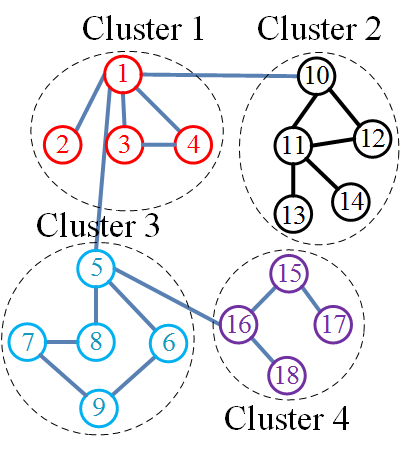
\includegraphics[scale=\scalefigure]{Pictures/CluMRCT/CluMRCT.png}
	\centering
	\caption{Cây khung phân cụm của bài toán CluMRCT cho đồ thị gồm 4 cụm và 18 đỉnh}
	\label{fig:vi_du_CluMRC}
\end{figure}

Hình \ref{fig:vi_du_CluMRC} minh họa cây khung phân cụm cho bài toán \gls{clumrct} của đồ thị đầu vào gồm 4 cụm, 18 đỉnh. Trong đó, các đỉnh thuộc một cụm nằm trong cùng một hình oval nét đứt.

\subsection{Bài toán Cây phân cụm đường đi ngắn nhất} \label{chap_coso:sec_mfea:subsec:cstp}
Bài toán \gls{cstp} được phát biểu như sau:

Cho một đơn đồ thị vô hướng $G = (V, E, w)$, một phân hoạch $R = \{R_1, R_2, R_3,\ldots,R_k\}$ của $V$ và đỉnh nguồn $s \in V$. Mục tiêu của bài toán \gls{cstp} là tìm một cây khung $T$ của đồ thị $G$ sao cho:
\begin{itemize}
	\item Với mỗi cụm $R_i (i=1,\ldots, k)$, đồ thị con $T[R_i]$ là một đồ thị liên thông.
	\item Tổng chi phí định tuyến giữa đỉnh nguồn và mỗi đỉnh $\sum_{v \in V(T)} d_T (s,v) \rightarrow$ min.
\end{itemize}

\renewcommand{\scalefigure}{0.6}
\begin{figure}[htbp]
	\centering		
	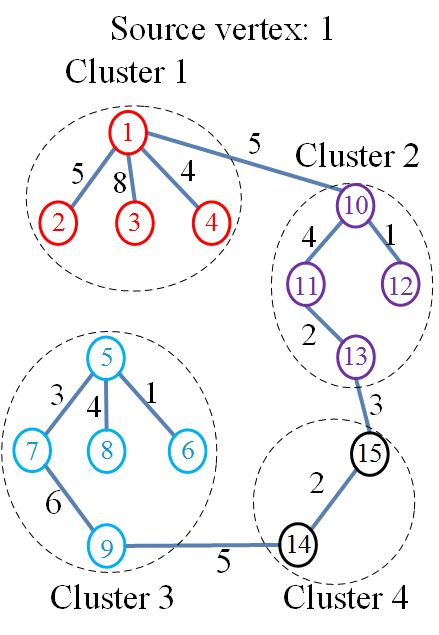
\includegraphics[scale=\scalefigure]{Pictures/CSTP/CSTP.png}
	\centering
	\caption{Cây khung phân cụm của bài toán \gls{cstp} cho đồ thị gồm 4 cụm và 15 đỉnh}
	\label{fig:vi_du_CSTP}
\end{figure}

Hình \ref{fig:vi_du_CSTP} minh họa một cây phân cụm của bài toán \gls{cstp} với đồ thị đầu vào gồm 15 đỉnh, 4 cụm và đỉnh 1 là đỉnh nguồn. Chi phí  của cây khung phân cụm là 186


%%=========--------------------------3. Các nghiên cứu liên quan---------------------------===============
\section{Các nghiên cứu liên quan} \label{chap_coso:sec:cacNghienCuuLienQuan}
\glsreset{clumrct}
\glsreset{cstp}
\glsreset{mfea}
Các bài toán liên quan đến các đỉnh được phân vào các cụm của đồ thị đã được biết đến từ những năm 70 của thế kỷ trước. Một trong các bài toán liên quan tới các đỉnh được phân cụm được nghiên cứu sớm nhất là bài toán \gls{clutsp}~\cite{bao_improved_2012, helsgaun_solving_2011, mestria_grasp_2013} - một biến thể của bài toán tối ưu tổ hợp nổi tiếng \gls{tsp} \cite{reinelt1994traveling}. Hiện nay, xuất phát từ yêu cầu cần tối ưu hệ thống mạng, bài toán cây phân cụm (clustered tree problems) nhận được nhiều sự quan tâm nghiên cứu.

Một trong các bài toán nhận được nhiều sự quan tâm nhất là bài toán \gls{clusteinertp}~\cite{wu_clustered_2015} - một biến thể của bài toán \gls{stp}~\cite{ihler_class_1999, winter1997euclidean}. Trong bài toán \gls{clusteinertp} các đỉnh cũng đươc chia vào các cụm, bài toán \gls{stp} là bài toán \gls{clusteinertp} nếu các cụm không có phần tử chung~\cite{wu2014clustered}. Trong \cite{wu_clustered_2015}, dựa trên kết quả thực nghiệm, các tác giả B. Y. Wu và C. W. Lin đã chỉ ra rằng tỉ lệ Steiner nằm trong khoảng (3,4) đem đến những kết quả có lợi nhất và từ đó đề xuất một giải thuật gần đúng cho bài toán \gls{clusteinertp} . Giải thuật này chuyển bài toán ban đầu về một bài toán cây Steiner sao cho cây Steiner tìm được không có đỉnh Steiner nào thuộc vào cây cục bộ của các cụm. Giải thuật được đề xuất giải có độ phức tạp đa thức.

Một biến thể khác của bài toán cây phân cụm, bài toán \gls{clumrct}~\cite{lin_minimum_2016}, trong nghiên cứu của mình các tác giả đã chỉ ra rằng bài toán \gls{clumrct} là NP-Khó nếu \gls{clumrct} có ít nhất 2 cụm. Nghiên cứu cũng đã đề xuất một giải thuật xấp xỉ cận tỉ lệ là 2 (2-approximation) để giải bài toán \gls{clumrct} bằng cách tạo đồ thị gồm 2 mức dựa trên cây khung R-star (R-star spanning tree) và dựa trên hai đặc trưng của cây khung \text{R-star}: một cây khung R-star với chi phí định tuyến nhỏ nhất có thể được tạo trong $O(n^2)$ với n là số đỉnh của bài toán và tồn tại một cây khung R-star với chi phí lớn nhất gấp 2 lần chi phí của lời giải tối ưu của bài toán \gls{clumrct}.


Gần đây, tác giả D'Emidio và các cộng sự \cite{demidio_clustered_2016} đã nghiên cứu một dạng khác của bài toán cây khung phân cụm, bài toán \gls{cstp}. Bài toán \gls{cstp} xuất hiện nhiều trong các ứng dụng cần tối ưu về thiết kế mạng, kết nối hệ thống cáp TV và hệ thống cáp quang. Trong nghiên cứu của mình nhóm tác giả đã đề xuất một giải thuật gần đúng (approximation algorithm - AAL) để giải bài toán \gls{cstp}. Ý tưởng chính của giải thuật AAL lần lượt tìm cây khung nhỏ nhất cho đồ thị con được cảm sinh từ tập đỉnh của mỗi cụm và đồ thị được nhận được bằng cách coi mỗi cụm là một đỉnh.

Như đã đề cập tới ở trong chương \ref{Chap_CoSoLyThuyet}, hướng tiếp cận sử dụng giải thuật gần đúng sẽ phù hợp hơn khi sử dụng giải các bài toán NP-Khó với dữ liệu đầu vào có kích thước lớn. Đối với các giải thuật gần đúng, giải thuật \gls{mfea} nổi lên như một giải thuật hiệu quả trong việc ứng dụng giải nhiều lớp bài toán khác nhau, đặc biệt các ứng dụng có hạn chế về tài nguyên sử dụng. Một trong các thế mạnh của giải thuật \gls{mfea} so với giải thuật GA là \gls{mfea} có thể tìm lời giải đồng thời của nhiều bài toán khác nhau nhưng chỉ sử dụng một mã hóa cá thể duy nhất cho tất cả các bài toán. Chính vì thế cho nên khi sử dụng giải thuật \gls{mfea}, lời giải của từng bài toán nhận được trên cơ sở thông tin của cá thể trong không gian \gls{uss}. Do đó, để sử dụng giải thuật \gls{mfea}, một trong các bước quan trọng cần phải giải quyết là tìm ra quy tắc biến đổi từ cá thể trong không gian \gls{uss} thành lời giải của từng bài toán. 

Hiện nay, giải thuật \gls{mfea} ngày càng khẳng định được vai trò là một công cụ mạnh trong việc tìm lời giải của nhiều bài toán lý thuyết và các ứng dụng thực tế. Tác giả Yuan,~Y. và các cộng sự~\cite{yuan2016evolutionary} đã đề xuất pháp pháp giải mã cho các bài toán tối ưu tổ hợp có biểu diễn hoán vị. Phương pháp đề xuất sẽ giữ lại các gen có giá trị nhỏ hơn kích thước của bài toán cần tìm lời giải, thứ tự của các gen được giữ lại là thứ tự xuất hiện trong không gian \gls{uss}. Trong nghiên cứu này, các tác giả còn đề xuất phương pháp lựa chọn cá thể theo mức (level-based selection methods - LSM) để lựa chọn cá thể tham gia vào quá trình tiến hóa ở thế hệ tiếp theo. Phương pháp LSM sẽ phân các cá thể vào các mức dựa trên tác vụ phù hợp nhất (skill factor) của cá thể đó. Các cá thể nào ở mức thấp hơn sẽ được ưu tiên chọn lọc cho thế hệ tiếp theo. Tác giả Feng,~L. và đồng nghiệp~\cite{feng2017empirical} đề xuất mô hình tiến hóa đa nhân tố cho giải thuật \gls{de} và giải thuật \gls{pso}. Đóng góp lớn nhất của các tác giả trong 2 giải thuật mới này là đã đề xuất các cơ chế xác định yếu tố ghép đôi cùng loại cho các cá thể con.


%----------------






%%================------------------Chap_mfeaGiaiCayPhanCum-------------------=============
\chapter{Giải thuật tiến hóa đa nhiệm giải bài toán cây khung phân cụm có chi phi định tuyến nhỏ nhất và bài toán cây phân cụm đường đi ngắn nhất}
\label{Chap_mfeaGiaiCayPhanCum}
%%=================--------------------------------3.Giai thuat de xuat---------------------------========================
Chương \ref{Chap_mfeaGiaiCayPhanCum} sẽ đề xuất một giải thuật tiến hóa đa nhân tố CluMFEA đa nhiệm giải đồng thời bài toán CluMRCT và bài toán CSPT. Giải thuật CluMFEA đề xuất gồm có hai tác vụ, một tác vụ CluMRCT và một tác vụ CSPT. Sơ đồ của giải thuật CluMFEA này giống với giải thuật MFEA cơ bản như đã trình bày ở mục 1.2.4. Nội dung đề xuất mới bao gồm đề xuất về biểu diễn cá thể, khởi tạo quần thể, các toán tử lai ghép, đột biến cho CluMFEA giải hai bài toán cụ thể là CluMRCT và CSPT.

Ngoài ra, đồ án cũng đề xuất một giải thuật di truyền CluGA giải hai bài toán CluMRCT và CSPT. Vì là giải thuật đơn nhiệm nên CluGA chỉ có thể giải lần lượt từng bài trong hai bài toán CluMRCT và CSPT. Sơ đồ của giải thuật CluGA đề xuất giống với sơ đồ giải thuật di truyền đã nêu ở mục 1.1 của chương 1. Nội dung đề xuất mới bao gồm cách biểu diễn cá thể và các toán tử khởi tạo, lai ghép, đột biến. Các đề xuất này giống với các đề xuất về các toán tử tương ứng cho CluMFEA.

Phần sau trình bày lần lượt các nội dung đề xuất.



%%=================--------------------------------1.Biểu diễn cá thể---------------------------========================
\section{Biểu diễn cá thể} \label{chap_mfeaProposed:sec:bieudiencathe}
Biểu diễn cá thể (hay mã hóa lời giải) đóng vai trò quan trọng trong các giải thuật tiến hóa, bởi nó ảnh hưởng trực tiếp tới việc lựa chọn và xây dựng các toán tử tiến hóa. Do đó, biểu diễn cá thể cũng ảnh hưởng lớn tới hiệu quả của giải thuật CluMFEA và CluGA được đề xuất. Có rất nhiều cách để biểu diễn cá thể là cây khung như sử dụng mã Dandelion~\cite{perfecto_dandelion_encoded_2016}, mã Blob~\cite{julstrom2005blob},.. Tuy nhiên, nhiều nghiên cứu đã chỉ ra rằng mã hóa cây khung sử dụng tập cạnh là một trong các mã hóa hiệu quả nhất trong các bài toán tìm cây khung~\cite{julstrom_initialization_2002, raidl_edge_2003, rothlauf_representations_2008}. Vì vậy, trong đồ án này, mã hóa tập cạnh được sử dụng để biểu diễn lời giải của hai bài toán CluMRCT và CluSTP.


\renewcommand{\scalefigure}{0.5}
\begin{figure}[htbp]
	\centering		
	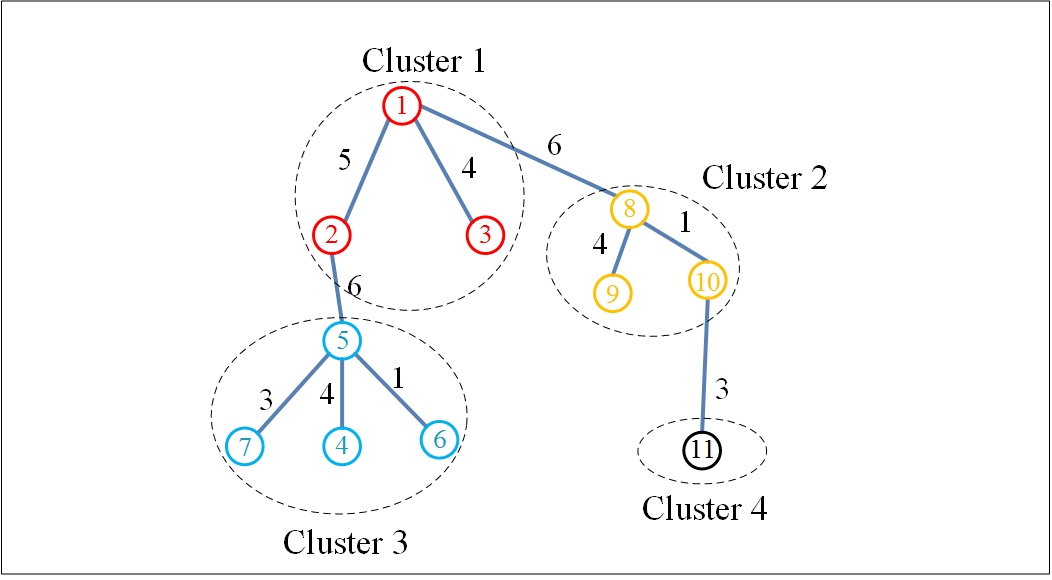
\includegraphics[scale=\scalefigure]{Pictures/Ind_representation/Ind_Representation.png}
	\centering
	\caption{Lời giải hợp lệ của bài toán CluMRCT và bài toán CSPT}
	\label{fig:ind_representation}
\end{figure}

Giả sử đồ thị trong hình~\ref{fig:ind_representation} là một lời giải hợp lệ của bài toán \gls{clumrct} và bài toán \gls{cstp}. Khi đó mã hóa tập cạnh tương ứng với lời giải này là \{(1,2); (1,3); (1,8); (2,5); (4,5); (5,7); (5,6); (8,9); (8,10); (10,11)\}.


%%=======--------------------------------2.	Khởi tạo quần thể---------------------------======
\section{Khởi tạo quần thể} \label{chap_mfeaProposed:sec:khoitaoquanthe}
Lời giải hợp lệ của bài toán \gls{cstp} và \gls{clumrct} là một cây khung T và các đồ thị cảm sinh của T trên mỗi cụm cũng là cây khung. Do đó, đồ án đề xuất một phương pháp khởi tạo ngẫu nhiên các cá thể luôn thỏa mãn các điều kiện ràng buộc của hai bài toán.

Các bước của giải thuật khởi tạo quần thể được trình bày trong thuật toán \ref{alg:DeXuatKhoiTaoCaThe}.
\begin{algorithm}[htb]
		\KwIn{Đồ thị $G=(V, E, w)$ và phân hoạch $R = \{R_1, R_2, R_3,\ldots,R_k\}$ của $V$}
		\KwOut{Một cây khung phân cụm $T_r=(V_r,E_r)$ của $G$}
		\BlankLine
	\Begin
	{	
		$V_r \leftarrow V$\;
		$G' \leftarrow$ H-Graph của đồ thị $G$\;
		$T' \leftarrow$ PrimRST($G'$) \Comment{Tạo cây khung ngẫu nhiên cho đồ thị H-Graph}\;
		\ForEach{cụm i-th}
		{
			$T_i \leftarrow$ PrimRST($G[R_i]$) \Comment{Tạo cây khung ngẫu nhiên cho cụm i}\;
		}
		$E_r \leftarrow \left( \cup_{i=1}^{k} E(T_i) \right)\cup E(T')$ \Comment{Hợp tập cạnh của cây khung của H-Graph và các cụm}\;
	}
	\caption{Khởi tạo một cá thể ngẫu nhiên}
	\label{alg:DeXuatKhoiTaoCaThe}
\end{algorithm}

%%=================--------------------------------3.Toán tử tiến hóa---------------------------========================
\section{Toán tử tiến hóa} \label{chap_mfeaProposed:sec:ToanTuTienHoa}
Toán tử lai ghép và đột biến được đề xuất luôn tạo ra cá thể hợp lệ cho cả hai bài toán \gls{clumrct} và bài toán \gls{cstp}. Chi tiết về các toán tử tiến hóa được trình bày dưới đây.

\subsection{Toán tử lai ghép} \label{chap_coso:sec_mfea:subsec:toantulaighep}
Trong toán tử lai ghép được đề xuất, các cạnh trên cá thể con đều được kế thừa từ các cạnh của một trong hai cá thể cha mẹ. Những cạnh xuất hiện ở cả 2 cá thể cha và cá thể mẹ sẽ chắc chắc được kế thừa ở cá  thể con. Điều này giúp đảm bảo việc lưu giữ các đặc điểm di truyền tốt cho thế hệ sau.

Các bước của toán tử lai ghép được trình bày trong thuật toán \ref{alg:laighepmoi}.
\begin{algorithm}[htb]
	\KwIn{Đồ thị $G=(V, E, w)$ và phân hoạch $R = \{R_1, R_2, \ldots,R_k\}$ của $V$; 
	\qquad \quad Cá thể cha mẹ: $T_{m}=\left(V,E_{m}\right), m = 1,2$.}
	\KwOut{Cá thể con $T_c = (V_c, E_c)$}
	\BlankLine
	\Begin
	{	
		$V_c \leftarrow V$\;
		\ForEach{cụm i-th}
		{
			$E_i \leftarrow E(T_1[R_i]) \cup E(T_2[R_i])$ \Comment{Hợp tập cạnh của cá thể cha mẹ của cụm i}\;
			$T_i \leftarrow$ PrimRST($(R_i, E_i$)) \Comment{Tạo cây khung ngẫu nhiên cho cụm i}\;
		}
		$T'_m \leftarrow$ H-Graph của đồ thị $T_m, m = 1,2$\;
		$T' \leftarrow$ PrimRST($T'_1 \cup T'_2$) \Comment{Tạo cây khung ngẫu nhiên cho đồ thị H-Graph}\;
		
		$E_c \leftarrow \left( \cup_{i=1}^{k} E(T_i) \right)\cup E(T')$ \Comment{Hợp tập cạnh của cây khung của H-Graph và các cụm}\;
	}
	\caption{Toán tử lai ghép mới}
	\label{alg:laighepmoi}
\end{algorithm}

\renewcommand{\scalefigure}{0.2}
\begin{figure}[tb]
	\centering	
	\setlength\tabcolsep{0 pt}
	\begin{tabular}{ccc}
		\renewcommand{\scalefigure}{0.203}
		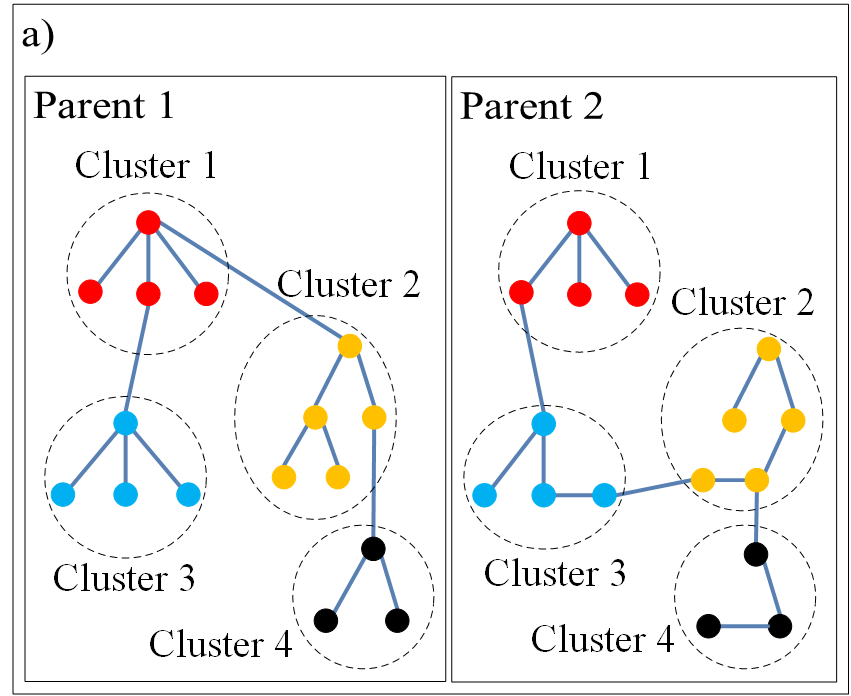
\includegraphics[scale=\scalefigure]{Pictures/Crossover/Crossover_New_a.png} &
		\renewcommand{\scalefigure}{0.20} 	
		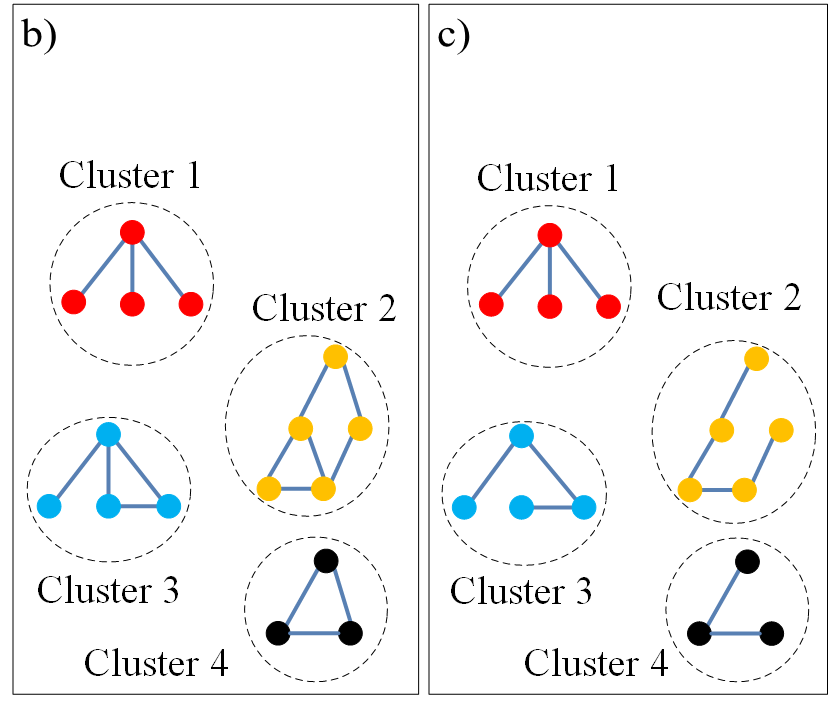
\includegraphics[scale=\scalefigure]{Pictures/Crossover/Crossover_New_b_c.png} &  
		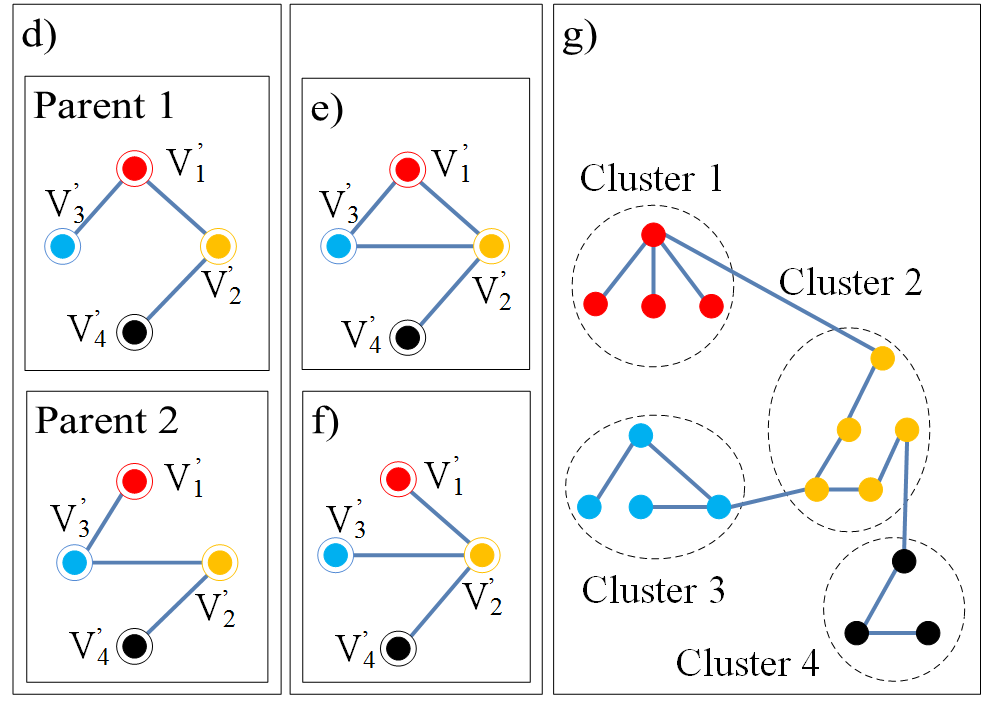
\includegraphics[scale=\scalefigure]{Pictures/Crossover/Crossover_New_d_e_f_g.png}\\
	\end{tabular}
	\centering
	\caption{Các bước lai ghép trong giải thuật MFEA đề xuất}
	\label{fig:Steps_of_novel_crossover_operator}
\end{figure}

Hình~\ref{fig:Steps_of_novel_crossover_operator} mô phỏng các bước của toán tử lai ghép trên. Trong đó,  Hình~\ref{fig:Steps_of_novel_crossover_operator}.a biểu diễn cá thể cha và cá thể mẹ trước khi được lai ghép. Đồ thị con của mỗi cluster sau khi hợp các cạnh của 2 cá thể cha mẹ được minh họa trong hình~\ref{fig:Steps_of_novel_crossover_operator}.b. Hình \ref{fig:Steps_of_novel_crossover_operator}.c minh họa các cây khung được tạo từ các đồ thị trong hình~\ref{fig:Steps_of_novel_crossover_operator}.b. sau khi áp dụng thuật toán PrimRST. Hình~\ref{fig:Steps_of_novel_crossover_operator}.d minh họa các H-Graph tương với các cá thể cha mẹ. Hình~\ref{fig:Steps_of_novel_crossover_operator}.e minh họa đồ thị nhận được sau khi hợp các H-Graph. Hình~\ref{fig:Steps_of_novel_crossover_operator}.f minh họa cây khung nhận được từ đồ thị trong Hình~\ref{fig:Steps_of_novel_crossover_operator}.e. sau khi áp dụng thuật toán PrimRST. Cá thể con được tao thành từ 2 cá thể cha mẹ được minh họa trong Hình~\ref{fig:Steps_of_novel_crossover_operator}.g.


\subsection{Toán tử đột biến} \label{chap_coso:sec_mfea:subsec:toantudotbien}
Ý tưởng chính của toán tử đột biến được tạo là tạo ra chu trình trên cá thể cha sau đó xóa bỏ cạnh trong chú trình đó để tạo thành cá thể mới hợp lệ.

Các bước của toán tử đột biến được trình bày trong thuật toán \ref{alg:dotbienmoi}.
\begin{algorithm}[htbp]
%	\SetAlgorithmName{MegaAlgorithm}{} %last arg is the title of listing table
%	\floatname{algorithm}{MegaAlgorithm}
	\KwIn{Cây khung $T_c$ của đồ thị G}
	\KwOut{Một cây khung con T}
	\BlankLine
	\Begin
	{	
		$R_i \leftarrow$ Chọn một cụm ngẫu nhiên của G\;
		$e \leftarrow$ Chọn cạnh ngẫu nhiên thuộc tập E($G[R_i]$) $\backslash$ E($T_c$)\;
		Thêm $e$ vào $T_c$ để tạo thành một chu trình $C$ trên $T_c$\;
		Xóa ngẫu nhiên cạnh $e' \in C$ thỏa mãn $e \neq e'$ \;
	}
	\caption{Toán tử Đột biến}
	\label{alg:dotbienmoi}
\end{algorithm}

Hình~\ref{fig:Illustation_of_new_mutation_operator} mô phỏng các bước trong thủ tục đột biến được đề xuất. Hình~\ref{fig:Illustation_of_new_mutation_operator}.a là cây khung $T_c$ trước khi bị đột biến. Hình~\ref{fig:Illustation_of_new_mutation_operator}.b minh họa đồ thị sau khi cụm thứ 3 (nền màu vàng) được chọn ngẫu nhiên. Hình~\ref{fig:Illustation_of_new_mutation_operator}.c minh họa đồ thị sau khi cạnh được thêm vào (cạnh nét đậm mầu đỏ) cụm thứ 3 để tạo thành chu trình. Hình~\ref{fig:Illustation_of_new_mutation_operator}.d minh họa đồ thị là kết quả của phép đột biến  sau khi một cạnh ngẫu nhiên khác cạnh vừa được thêm vào được loại bỏ khỏi $T_c$.

\renewcommand{\scalefigure}{0.26}
\begin{figure}[htb]
	\centering	
	\setlength\tabcolsep{0 pt}
	\begin{tabular}{cc}
		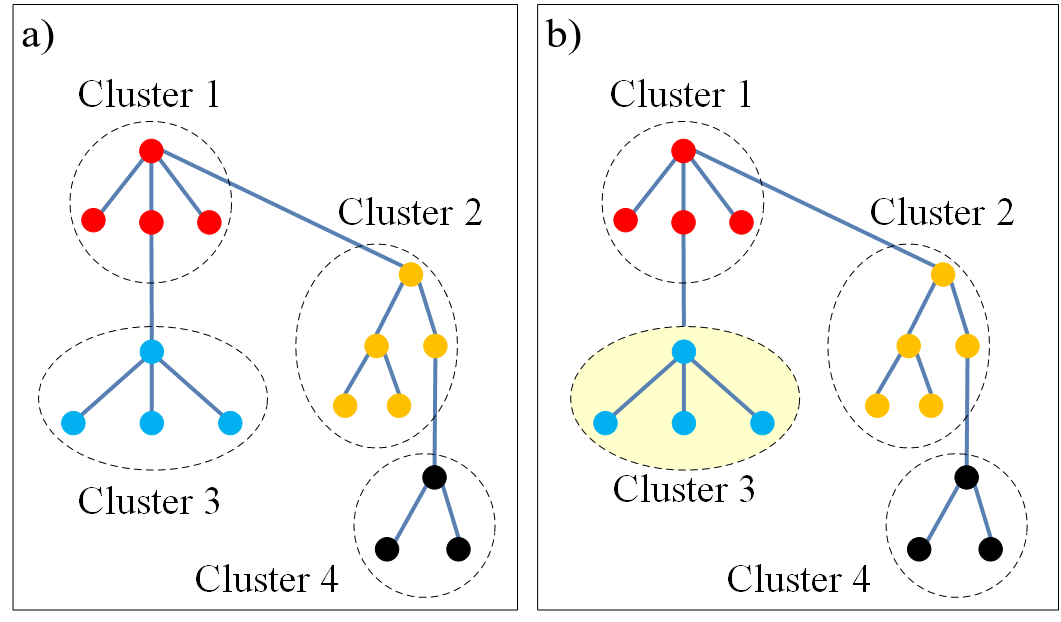
\includegraphics[scale=\scalefigure]{Pictures/Mutation/Mutation_a_b.png} & 	
		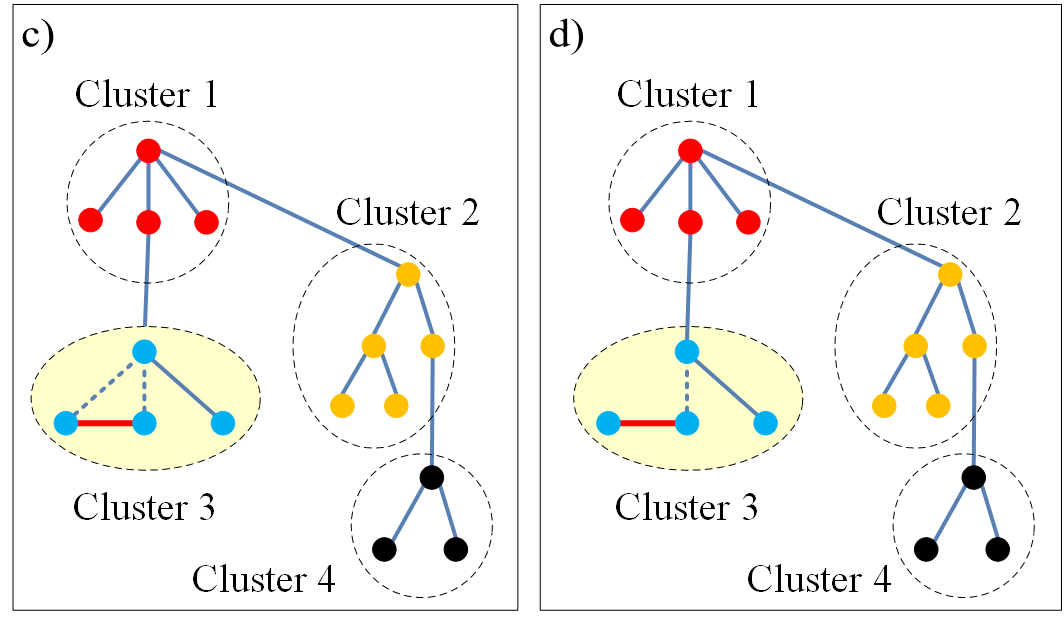
\includegraphics[scale=\scalefigure]{Pictures/Mutation/Mutation_c_d.png} \\
	\end{tabular}
	\centering
	\caption{Ví dụ minh họa toán tử đột biến mới}
	\label{fig:Illustation_of_new_mutation_operator}
\end{figure}


%%=================--------------------------------5.	Phương pháp giải mã cá thể---------------------------========================
\section{Phương pháp giải mã cá thể} \label{chap_mfeaProposed:sec:dexuatgiaima}
Đồ án có mục tiêu giải hai bài toán \gls{clumrct} và \gls{cstp}, nên giải thuật \gls{mfea} xác định lời giải của mỗi bài toán từ \gls{uss}. Do đầu vào của hai bài toán giống nhau và đầu ra đều là cây khung phân cụm (nhưng hàm mục tiêu khác nhau) nên cá thể trong \gls{uss} cũng là lời giải hợp lệ cho cả bài toán trên. Do đó, phép  giải mã chỉ đơn giản là lấy thông tin cá thể trong không gian \gls{uss}. 





%%================------------------Chap_kqThucNghiem-------------------=============
\chapter{Kết quả thực nghiệm}
\label{Chap_kqThucNghiem}
%%=====-------------------------------- 1. Dữ liệu thực nghiệm --------------------------====
\section{Dữ liệu thực nghiệm} \label{chap_mfeaProposed:sec:dulieuthucnghiem}

Phần thực nghiệm của đồ án sử dụng dữ liệu là 6 tập dữ liệu chuẩn MOM của bài toán người đi du lịch phân cụm Euclid (Euclidean Clustered Travelling Salesman problem) được công bố trong  [9] bởi M. Mestria và các cộng sự. Các tập dữ liệu này phù hợp cho các bài toán về cây phân cụm.

Các tập dữ liệu MOM có thể được tải xuống từ địa chỉ \url{http://www.akira.ruc.dk/~keld/research/CLKH/MOM.tgz}. Các bài toán đầu vào thuộc bộ dữ liệu được phân loại dựa trên số đỉnh của đồ thị, bao gồm 3 tập dữ liệu loại nhỏ (Type Small) và 3 tập dữ liệu loại lớn (Type Large). Kích thước của các bài toán thuộc 3 tập nhỏ là từ 30 đến 120 đỉnh. Kích thước các bài toán thuộc 3 tập lớn là từ 260 đến 300 đỉnh.

Do đầu vào của bài toán CSPT cần thêm thông tin về đỉnh nguồn, các bộ dữ liệu đã được điều chỉnh để phù hợp với bài toán. Cụ thể, một đỉnh được chọn ngẫu nhiên trong các đỉnh có sẵn để làm đỉnh nguồn và thêm vào trong mỗi bộ dữ liệu.

Trong giới hạn của đồ án, giải thuật được thực nghiệm trên 3 bộ dữ liệu loại nhỏ của MOM là các tập Type 1, Type 5 và Type 6. Các bộ dữ liệu này cùng với thông tin về đỉnh nguồn đã được thêm vào có thể tìm thấy tại  \url{https://drive.google.com/drive/folders/1owpNkxvhIc6jqyr54w2KvyIV2RTaAH-p?usp=sharing}.

 
 %%=================--------------------------------  3.	Môi trường thực nghiệm ---------------------------========================
\section{Nội dung thực nghiệm} \label{chap_mfeaProposed:sec:caidatthucnghiem}
Thực nghiệm sẽ cài đặt giải thuật CluMFEA và CluGA đã đề xuất ở Chương 3 để giải bài toán CluSPT và bài toán CluMRCT.

Chương trình cài đặt giải thuật CluMFEA gồm hai tác vụ, một tác vụ CSPT và một tác vụ CluMRCT. Nói cách khác, một chương trình CluMFEA sẽ giải đồng thời cả hai bài toán. Trong khi đó, giải thuật CluGA sẽ được cài đặt thành hai chương trình: một chương trình CluGA giải bài toán CluSPT và một chương trình CluGA giải bài toán CluMRCT. 

Mục đích của thực nghiệm này là so sánh hiệu quả của giải thuật CluMFEA so với CluGA đối với từng bài toán. Giá trị hàm mục tiêu (chi phí) và thời gian chạy sẽ được tổng hợp, thống kê, phân tích và đánh giá. Các kết quả được trình bày trong phần Kết quả thực nghiệm.

Để có thể có được sự đánh giá chính xác đối với hai giải thuật CluMFEA và CluGA, những tham số thực nghiệm sau sẽ được sử dụng:
\begin{itemize}
	\item 	$nInds$ – Số cá thể trong quần thể tiến hóa của mỗi thế hệ
	\item $nGens$ – Số thế hệ
	\item $nTasks$ – Số tác vụ của giải thuật
	\item $nET$– Số tác vụ được đánh giá cho mỗi cá thể trong một thế hệ
	\item $nEvals$ – Tổng số phép đánh giá cá thể của giải thuật, được tính bằng công thức: $nEvals=nInds* nGens *nET$
	\item $rmp$ – Xác suất ghép đôi ngẫu nhiên của CluMFEA
	\item $cRate$ – Xác suất lai ghép của CluGA
	\item $mRate$ – Xác suất đột biến của CluGA
	\item $nRuns$ – Số lần chạy
\end{itemize}

%\setlength{\intextsep}{3pt}

%\setlength{\intextsep}{1pt} 

Tham số của thực nghiệm cho từng giải thuật được cho trong bảng dưới đây:
\begin{center}
	\begin{tabular}{p{4.8cm} p{5.3cm} c}	
		\hline 
			 & CluMFEA & CluGA \\ 
		\hline 
		$nInds$	 & 100 & 100 \\ 
		\hline
		$nGens$ & 500 & 500 \\
		\hline 
		$nTasks$ & 2 & 1 \\
		\hline
		$nET$ & 1 & 1 \\
		\hline 
		$nEvals$ & 50000 & 50000 \\ 
		\hline 
		$rmp$ & 0.2 & \\ 
		\hline 
		$mRate$ & & 0.6 \\ 
		\hline 
		$cRate$ & & 0.02 \\  
		\hline 
		$nRuns$ & 20 & 20 \\
		\hline
	\end{tabular} 
\end{center} 
  
  
%%=================-------------------------------- 2.	Nội dung thực nghiệm ---------------------------========================
%\section{Nội dung thực nghiệm} \label{chap_mfeaProposed:sec:noidungthucnghiem}

Các tham số về số cá thể, số thế hệ, số phép tính toán được lựa chọn sao cho sự so sánh giữa CluMFEA với CluGA này là hợp lý và có nhiều ý nghĩa. Xác suất lai ghép của CluGA được lựa chọn cho thử nghiệm dựa trên tỉ lệ rmp của CluMFEA bằng cách tính sau: Trong MFEA cơ bản và CluMFEA, do các cá thể chỉ được lai ghép nếu cặp cha mẹ có chung skill factor hoặc nằm trong số một tỉ lệ rmp những cá thể còn lại. Giả định các yếu tố thực nghiệm có tính khách quan cao và thực hiện với số lần đủ nhiều, xác suất cặp cha mẹ có skill factor giống nhau là 0.5. Khi đó xác suất lai ghép sẽ là 0.5+rmp*0.5.

Giải thuật CluMFEA đề xuất được cài đặt với tham số rmp = 0.2 nên xác suất lai ghép tương ứng của CluGA được chộn là 0.5+0.2*0.5=0.6. Xác suất đột biến của các giải thuật GA truyền thống thường được chọn rất nhỏ. Do đó, trong thực nghiệm này xác suất của CluGA được chọn là 0.02, nằm trong khoảng có thể chấp nhận.

\section{Môi trường thực nghiệm}
Môi trường: Hệ điều hành Windows 8 Ultimate-64 bit.

Thông số phần cứng:
\begin{itemize}
\item Bộ vi xử lý: Intel Core i7-3.6 GHz.
\item RAM: 16GB
\end{itemize}

 %%=================--------------------------------  3.	Kết quả thực nghiệm ---------------------------========================
\section{Kết quả thực nghiệm} \label{chap_mfeaProposed:sec:ketqua}
Để phục vụ cho việc so sánh hiệu quả hai giải thuật, dữ liệu về giá trị hàm mục tiêu (ở đây là chi phí) và thời gian thu được sử dụng để tính toán các giá trị sau:

\begin{itemize}
	\item Min – Giá trị hàm mục tiêu nhỏ nhất trong 20 lần chạy
	\item Mean – Giá trị trung bình của hàm mục tiêu sau 20 lần chạy
	\item Max – Giá trị hàm mục tiêu lớn nhất trong 20 lần chạy
	\item Std – Độ lệch chuẩn của các giá trị hàm mục tiêu trong 20 lần chạy
	\item Time – Thời gian chạy trung bình của 20 lần chạy
	
\end{itemize}

\subsection{So sánh kết quả CluMFEA và CluGA đối với bài toán CluSPT}
Kết quả thực nghiệm cho thấy CluMFEA cho lời giải trung bình tốt hơn CluGA trên 48/85 bài toán đầu vào của 3 tập dữ liệu Type 1, Type 5, Type 6. 

Có thể dễ dàng nhận thấy một hiện tượng bất thường: CluMFEA vượt trội hơn CluGA ở 20/21 bài toán đầu vào của Type 5, nhưng lại kém hơn CluGA ở hơn một nửa số bài toán trong hai tập còn lại. Các bài toán đầu vào trong mỗi tập dữ liệu của MOM được tạo ra bằng cùng một thuật toán và thường mang đặc điểm chung nào đó [10]. Do đó, một câu hỏi được đặt ra là phải chăng tồn tại ít nhất một yếu tố nào đó chi phối mức độ vượt trội của CluMFEA so với CluGA, hay nói cách khác là chi phối hiệu quả của hai giải thuật khi giải bài toán CSPT.
 
Sau đây là kết quả  cụ thể trên 3 tập dữ liệu:   


\subsection{So sánh kết quả CluMFEA và CluGA đối với bài toán CluMRCT}




%%================------------------Chap_Ketluan-------------------=============
\chapter{Kết luận}
\label{Chap_Ketluan}
Đồ án đã trình bày những nội dung sau:
\begin{itemize}
	\item Trình bày tổng quát nội dung của các giải thuật di truyền và các phương pháp phổ biến được áp dụng cho giải thuật.
	\item Trình bày về giải thuật MFEA cơ bản và các nhân tố trong giải thuật.
	\item Khái quát mô hình hai bài toán CluSPT và CluMRCT.
	\item Đề xuất một giải thuật CluMFEA và để giải đồng thời hai bài toán CSPT và CluMRCT bao gồm đề xuất mã hóa cá thể, lai ghép, đột biến.
	\item Đề xuất một giải thuật CluGA đơn nhiệm với cùng cách mã hóa cá thể và các toán tử lai ghép, đột biến với CluMFEA để giải bài toán CSPT và CluMRCT.
\end{itemize}
Đồ án đã thu được những kết quả thực nghiệm sau:
\begin{itemize}
	\item Cài đặt thành công giải thuật CluMFEA và CluGA đã đề xuất.
	\item Chạy thử nghiệm CluMFEA đa nhiệm giải đồng thời hai bài toán CSPT và CluMRCT.
	\item Chạy thử nghiệm CluGA đơn nhiệm lần lượt đối với từng bài toán CSPT và CluMRCT. 
	\item Tập hợp kết quả so sánh hai giải thuật trên các tập dữ liệu chuẩn, gồm tổng cộng 85 bộ dữ liệu, mỗi bộ chạy 20 lần.
	\item Tổng hợp kết quả và thực hiện các công việc thống kê, phân tích, đánh giá các kết quả thực nghiệm.
\end{itemize}

Kết quả thực nghiệm cho thấy giải thuật CluMFEA cho ra những kết quả vượt trội hơn CluGA ở một số bộ dữ liệu nhưng kém hơn ở một số bộ dữ liệu. Tuy nhiên, đồ án đã chỉ ra và chứng minh được một yếu tố quan trọng quyết định CluMFEA hay CluGA vượt trội hơn: đó là tỉ lệ giữa số cụm và số đỉnh của đồ thị đầu vào, hay dễ hiểu hơn là yếu tố liên quan đến số đỉnh trung bình của mỗi cụm. Giải thuật CluMFEA giải hai bài toán cùng một lúc có thời gian chạy bằng hoặc chỉ gần bằng thời gian chạy một bài toán đơn lẻ với CluGA, do ở mỗi thế hệ mỗi cá thể mới sinh ra chỉ được đánh giá với một tác vụ duy nhất thay vì với cả hai tác vụ CluMFEA, dẫn tới tổng số phép đánh giá của CluMFEA chỉ bằng chứ không gấp đôi của CluGA. Điều này là phù hợp với những phân tích về mặt lý thuyết đã trình bày trước đó.

Từ những phân tích trên, đồ án rút ra được giải thuật CluMFEA đã được đề xuất có ưu thế về mặt thời gian hơn so với giải thuật CluGA khi cần giải cả hai bài toán CSPT và CluMRCT. Về mặt chất lượng lời giải, giải thuật CluMFEA mang lại những kết quả tốt hơn đáng kể so với CluGA khi áp dụng cho những bài toán có tỉ lệ giữ số cụm và số đỉnh dưới 0.2. Tỉ lệ này càng tăng thì sự vượt trội so với CluGA càng giảm. Khi tỉ lệ vượt mức 0.2 thì đối với bài toán CSPT giải thuật CluMFEA đã đề xuất không đem lại nhiều lợi ích hơn so với CluGA, nhưng ở một số bộ dữ liệu CluMFEA giành được ưu thế khi giải bài CluMRCT. Điều đó cho thấy tỉ lệ số cụm/ số đỉnh không phải yếu tố quyết định duy nhất.
Do giới hạn của đồ án cũng như do những giới hạn về kiến thức, kinh nghiệm và kĩ năng của người thực hiện, đồ án chắc chắn còn tồn tại nhiều thiếu sót, ví dụ như:

\begin{itemize}
	\item Chưa thử nghiệm giải thuật CluMFEA và CluGA đã đề xuất với nhiều bộ tham số đầu vào khác nhau.
	\item Chưa khai thác được hết những nhận định có ích khác mà kết quả thực nghiệm có thể đem lại.
\end{itemize}
Một số hướng đi khả thi trong tương lai để phát triển đồ án như sau:
\begin{itemize}
	\item Thay đổi tham số đầu vào và chạy thử nghiệm nhiều lần.
	\item Đề xuất những toán tử di truyền mới cho giải thuật.
	\item Tìm hiểu những mối tương quan khác có thể ảnh hưởng tới hiệu quả của giải thuật, ví dụ như trọng số cạnh trung bình, độ dài đường đi trung bình,...
	\item Đề xuất giải thuật MFEA cho các bài toán khác.
\end{itemize}



\newpage
%\section*{References}


%\bibliographystyle{unsrt}
\bibliographystyle{plain}
\bibliography{references}

%\printbibliography



%\printglossaries
%\glsaddall



\end{document}